\documentclass[twoside]{book}

% Packages required by doxygen
\usepackage{fixltx2e}
\usepackage{calc}
\usepackage{doxygen}
\usepackage[export]{adjustbox} % also loads graphicx
\usepackage{graphicx}
\usepackage[utf8]{inputenc}
\usepackage{makeidx}
\usepackage{multicol}
\usepackage{multirow}
\PassOptionsToPackage{warn}{textcomp}
\usepackage{textcomp}
\usepackage[nointegrals]{wasysym}
\usepackage[table]{xcolor}

% NLS support packages
\usepackage[spanish]{babel}
% Font selection
\usepackage[T1]{fontenc}
\usepackage[scaled=.90]{helvet}
\usepackage{courier}
\usepackage{amssymb}
\usepackage{sectsty}
\renewcommand{\familydefault}{\sfdefault}
\allsectionsfont{%
  \fontseries{bc}\selectfont%
  \color{darkgray}%
}
\renewcommand{\DoxyLabelFont}{%
  \fontseries{bc}\selectfont%
  \color{darkgray}%
}
\newcommand{\+}{\discretionary{\mbox{\scriptsize$\hookleftarrow$}}{}{}}

% Page & text layout
\usepackage{geometry}
\geometry{%
  a4paper,%
  top=2.5cm,%
  bottom=2.5cm,%
  left=2.5cm,%
  right=2.5cm%
}
\tolerance=750
\hfuzz=15pt
\hbadness=750
\setlength{\emergencystretch}{15pt}
\setlength{\parindent}{0cm}
\setlength{\parskip}{3ex plus 2ex minus 2ex}
\makeatletter
\renewcommand{\paragraph}{%
  \@startsection{paragraph}{4}{0ex}{-1.0ex}{1.0ex}{%
    \normalfont\normalsize\bfseries\SS@parafont%
  }%
}
\renewcommand{\subparagraph}{%
  \@startsection{subparagraph}{5}{0ex}{-1.0ex}{1.0ex}{%
    \normalfont\normalsize\bfseries\SS@subparafont%
  }%
}
\makeatother

% Headers & footers
\usepackage{fancyhdr}
\pagestyle{fancyplain}
\fancyhead[LE]{\fancyplain{}{\bfseries\thepage}}
\fancyhead[CE]{\fancyplain{}{}}
\fancyhead[RE]{\fancyplain{}{\bfseries\leftmark}}
\fancyhead[LO]{\fancyplain{}{\bfseries\rightmark}}
\fancyhead[CO]{\fancyplain{}{}}
\fancyhead[RO]{\fancyplain{}{\bfseries\thepage}}
\fancyfoot[LE]{\fancyplain{}{}}
\fancyfoot[CE]{\fancyplain{}{}}
\fancyfoot[RE]{\fancyplain{}{\bfseries\scriptsize Generado por Doxygen }}
\fancyfoot[LO]{\fancyplain{}{\bfseries\scriptsize Generado por Doxygen }}
\fancyfoot[CO]{\fancyplain{}{}}
\fancyfoot[RO]{\fancyplain{}{}}
\renewcommand{\footrulewidth}{0.4pt}
\renewcommand{\chaptermark}[1]{%
  \markboth{#1}{}%
}
\renewcommand{\sectionmark}[1]{%
  \markright{\thesection\ #1}%
}

% Indices & bibliography
\usepackage{natbib}
\usepackage[titles]{tocloft}
\setcounter{tocdepth}{3}
\setcounter{secnumdepth}{5}
\makeindex

% Hyperlinks (required, but should be loaded last)
\usepackage{ifpdf}
\ifpdf
  \usepackage[pdftex,pagebackref=true]{hyperref}
\else
  \usepackage[ps2pdf,pagebackref=true]{hyperref}
\fi
\hypersetup{%
  colorlinks=true,%
  linkcolor=blue,%
  citecolor=blue,%
  unicode%
}

% Custom commands
\newcommand{\clearemptydoublepage}{%
  \newpage{\pagestyle{empty}\cleardoublepage}%
}

\usepackage{caption}
\captionsetup{labelsep=space,justification=centering,font={bf},singlelinecheck=off,skip=4pt,position=top}

%===== C O N T E N T S =====

\begin{document}

% Titlepage & ToC
\hypersetup{pageanchor=false,
             bookmarksnumbered=true,
             pdfencoding=unicode
            }
\pagenumbering{alph}
\begin{titlepage}
\vspace*{7cm}
\begin{center}%
{\Large Laboratorio de P\+R\+O2. Práctica \textquotesingle{}Codificador y decodificador de textos\textquotesingle{}. \\[1ex]\large Versión final 20-\/05-\/2019 }\\
\vspace*{1cm}
{\large Generado por Doxygen 1.8.13}\\
\end{center}
\end{titlepage}
\clearemptydoublepage
\pagenumbering{roman}
\tableofcontents
\clearemptydoublepage
\pagenumbering{arabic}
\hypersetup{pageanchor=true}

%--- Begin generated contents ---
\chapter{Entrega final\+: documentación completa.}
\label{index}\hypertarget{index}{}En esta práctica se construye un programa modular que ofrece un menú de opciones para gestionar un codificador y decodificador de textos en diversos idiomas. Se introducen las clases {\itshape \hyperlink{class_cjt__idiomas}{Cjt\+\_\+idiomas}}, {\itshape \hyperlink{class_idioma}{Idioma}} y {\itshape \hyperlink{class_tab_freq}{Tab\+Freq}}.

Se documenta la especificación y la implementación de los métodos públicos y los privados de cada clase. 
\chapter{Índice de clases}
\section{Lista de clases}
Lista de las clases, estructuras, uniones e interfaces con una breve descripción\+:\begin{DoxyCompactList}
\item\contentsline{section}{\hyperlink{class_cjt__idiomas}{Cjt\+\_\+idiomas} \\*Representa un conjunto de idiomas }{\pageref{class_cjt__idiomas}}{}
\item\contentsline{section}{\hyperlink{class_idioma}{Idioma} \\*Representa un idioma }{\pageref{class_idioma}}{}
\item\contentsline{section}{\hyperlink{class_tab_freq}{Tab\+Freq} \\*Representa una tabla de frecuencias de los carácteres de un idioma }{\pageref{class_tab_freq}}{}
\end{DoxyCompactList}

\chapter{Indice de archivos}
\section{Lista de archivos}
Lista de todos los archivos con descripciones breves\+:\begin{DoxyCompactList}
\item\contentsline{section}{\hyperlink{_cjt__idiomas_8cc}{Cjt\+\_\+idiomas.\+cc} \\*Implementación de la clase \hyperlink{_cjt__idiomas_8hh}{Cjt\+\_\+idiomas.\+hh} }{\pageref{_cjt__idiomas_8cc}}{}
\item\contentsline{section}{\hyperlink{_cjt__idiomas_8hh}{Cjt\+\_\+idiomas.\+hh} \\*Especificación de la clase \hyperlink{class_cjt__idiomas}{Cjt\+\_\+idiomas} }{\pageref{_cjt__idiomas_8hh}}{}
\item\contentsline{section}{\hyperlink{idioma_8cc}{idioma.\+cc} \\*Implementación de la clase \hyperlink{idioma_8hh}{idioma.\+hh} }{\pageref{idioma_8cc}}{}
\item\contentsline{section}{\hyperlink{idioma_8hh}{idioma.\+hh} \\*Especificación de la clase \hyperlink{class_idioma}{Idioma} }{\pageref{idioma_8hh}}{}
\item\contentsline{section}{\hyperlink{program_8cc}{program.\+cc} \\*Programa principal de la práctica }{\pageref{program_8cc}}{}
\item\contentsline{section}{\hyperlink{_tab_freq_8cc}{Tab\+Freq.\+cc} \\*Implementación de la clase \hyperlink{_tab_freq_8hh}{Tabfreq.\+hh} }{\pageref{_tab_freq_8cc}}{}
\item\contentsline{section}{\hyperlink{_tab_freq_8hh}{Tab\+Freq.\+hh} \\*Especificación de la clase \hyperlink{class_tab_freq}{Tab\+Freq} }{\pageref{_tab_freq_8hh}}{}
\end{DoxyCompactList}

\chapter{Documentación de las clases}
\hypertarget{class_cjt__idiomas}{}\section{Referencia de la Clase Cjt\+\_\+idiomas}
\label{class_cjt__idiomas}\index{Cjt\+\_\+idiomas@{Cjt\+\_\+idiomas}}


Representa un conjunto de idiomas.  


\subsection*{Métodos públicos}
\begin{DoxyCompactItemize}
\item 
\hyperlink{class_cjt__idiomas_acf95ab4c8f5fc442e3724a804658dd38}{Cjt\+\_\+idiomas} ()
\begin{DoxyCompactList}\small\item\em Creadora por defecto. \end{DoxyCompactList}\item 
\hyperlink{class_cjt__idiomas_acd4deb8546959ab728ce5c4bc717e800}{$\sim$\+Cjt\+\_\+idiomas} ()
\begin{DoxyCompactList}\small\item\em Destructora por defecto. \end{DoxyCompactList}\item 
void \hyperlink{class_cjt__idiomas_a1e38b16ba4bb49a91589c85ec7775a5f}{afegir\+\_\+mod\+\_\+idioma} (string \&key)
\begin{DoxyCompactList}\small\item\em Modificadora del conjunto de idiomas. \end{DoxyCompactList}\item 
void \hyperlink{class_cjt__idiomas_af3724a3343435acc48397c555722ce2f}{codifica\+\_\+I} (string \&key, string \&text) const
\begin{DoxyCompactList}\small\item\em Consultora de la codificación del texto introducido en un idioma contreto. \end{DoxyCompactList}\item 
void \hyperlink{class_cjt__idiomas_a99a44238cc4b83392ff1991ad1319c46}{decodifica\+\_\+I} (string \&key, string \&codi) const
\begin{DoxyCompactList}\small\item\em Consultora de la decodificación del código introducido en un idioma concreto. \end{DoxyCompactList}\item 
void \hyperlink{class_cjt__idiomas_a9839ea44dc8c3ecbb10b32fe869a3498}{print\+\_\+taula} (string key)
\begin{DoxyCompactList}\small\item\em Consultora de la tabla de frecuencias de un idioma del conjunto. \end{DoxyCompactList}\item 
void \hyperlink{class_cjt__idiomas_a0ac0bb2a2fe0cf4abd10d9366da9fa10}{print\+\_\+lista} (string key)
\begin{DoxyCompactList}\small\item\em Consultora de la lista de códigos de un idioma del conjunto. \end{DoxyCompactList}\item 
void \hyperlink{class_cjt__idiomas_afb0c806ea9fb7422f10d7767ef101743}{print\+\_\+code\+\_\+op} (string key, string key2)
\begin{DoxyCompactList}\small\item\em Consultora del código de un carácter de un idioma del conjunto. \end{DoxyCompactList}\item 
void \hyperlink{class_cjt__idiomas_abcb2442285737fae69096a5e05b9a594}{print\+\_\+\+I\+\_\+treecode} (string \&key)
\begin{DoxyCompactList}\small\item\em Consultora del treecode de un idioma del conjunto. \end{DoxyCompactList}\item 
void \hyperlink{class_cjt__idiomas_a09e45083b9df57c02f05bda0bef3d0d3}{read\+\_\+conjunto} (int n)
\begin{DoxyCompactList}\small\item\em Operación de lectura. \end{DoxyCompactList}\end{DoxyCompactItemize}
\subsection*{Atributos privados}
\begin{DoxyCompactItemize}
\item 
map$<$ string, \hyperlink{class_idioma}{Idioma} $>$ \hyperlink{class_cjt__idiomas_aeb67a7100b1345a160fb85466bd4e5f6}{C\+J\+\_\+\+ID}
\begin{DoxyCompactList}\small\item\em Estructura del conjunto de idiomas. \end{DoxyCompactList}\end{DoxyCompactItemize}


\subsection{Descripción detallada}
Representa un conjunto de idiomas. 

Definición en la línea 17 del archivo Cjt\+\_\+idiomas.\+hh.



\subsection{Documentación del constructor y destructor}
\mbox{\Hypertarget{class_cjt__idiomas_acf95ab4c8f5fc442e3724a804658dd38}\label{class_cjt__idiomas_acf95ab4c8f5fc442e3724a804658dd38}} 
\index{Cjt\+\_\+idiomas@{Cjt\+\_\+idiomas}!Cjt\+\_\+idiomas@{Cjt\+\_\+idiomas}}
\index{Cjt\+\_\+idiomas@{Cjt\+\_\+idiomas}!Cjt\+\_\+idiomas@{Cjt\+\_\+idiomas}}
\subsubsection{\texorpdfstring{Cjt\+\_\+idiomas()}{Cjt\_idiomas()}}
{\footnotesize\ttfamily Cjt\+\_\+idiomas\+::\+Cjt\+\_\+idiomas (\begin{DoxyParamCaption}{ }\end{DoxyParamCaption})}



Creadora por defecto. 

Se ejecuta automáticamente al declarar un conjunto de idiomas. \begin{DoxyPrecond}{Precondición}
{\itshape cierto} 
\end{DoxyPrecond}
\begin{DoxyPostcond}{Postcondición}
Crea un conjunto de idiomas 
\end{DoxyPostcond}
\begin{DoxyParagraph}{Coste}
Constante 
\end{DoxyParagraph}


Definición en la línea 9 del archivo Cjt\+\_\+idiomas.\+cc.


\begin{DoxyCode}
9 \{\}
\end{DoxyCode}
\mbox{\Hypertarget{class_cjt__idiomas_acd4deb8546959ab728ce5c4bc717e800}\label{class_cjt__idiomas_acd4deb8546959ab728ce5c4bc717e800}} 
\index{Cjt\+\_\+idiomas@{Cjt\+\_\+idiomas}!````~Cjt\+\_\+idiomas@{$\sim$\+Cjt\+\_\+idiomas}}
\index{````~Cjt\+\_\+idiomas@{$\sim$\+Cjt\+\_\+idiomas}!Cjt\+\_\+idiomas@{Cjt\+\_\+idiomas}}
\subsubsection{\texorpdfstring{$\sim$\+Cjt\+\_\+idiomas()}{~Cjt\_idiomas()}}
{\footnotesize\ttfamily Cjt\+\_\+idiomas\+::$\sim$\+Cjt\+\_\+idiomas (\begin{DoxyParamCaption}{ }\end{DoxyParamCaption})}



Destructora por defecto. 

Se ejecuta automáticamente cuando el objeto local sale del ámbito de visibilidad \begin{DoxyPrecond}{Precondición}
{\itshape cierto} 
\end{DoxyPrecond}
\begin{DoxyPostcond}{Postcondición}
El objeto local se ha borrado 
\end{DoxyPostcond}
\begin{DoxyParagraph}{Coste}
Constante 
\end{DoxyParagraph}


Definición en la línea 11 del archivo Cjt\+\_\+idiomas.\+cc.


\begin{DoxyCode}
11 \{\}
\end{DoxyCode}


\subsection{Documentación de las funciones miembro}
\mbox{\Hypertarget{class_cjt__idiomas_a1e38b16ba4bb49a91589c85ec7775a5f}\label{class_cjt__idiomas_a1e38b16ba4bb49a91589c85ec7775a5f}} 
\index{Cjt\+\_\+idiomas@{Cjt\+\_\+idiomas}!afegir\+\_\+mod\+\_\+idioma@{afegir\+\_\+mod\+\_\+idioma}}
\index{afegir\+\_\+mod\+\_\+idioma@{afegir\+\_\+mod\+\_\+idioma}!Cjt\+\_\+idiomas@{Cjt\+\_\+idiomas}}
\subsubsection{\texorpdfstring{afegir\+\_\+mod\+\_\+idioma()}{afegir\_mod\_idioma()}}
{\footnotesize\ttfamily void Cjt\+\_\+idiomas\+::afegir\+\_\+mod\+\_\+idioma (\begin{DoxyParamCaption}\item[{string \&}]{key }\end{DoxyParamCaption})}



Modificadora del conjunto de idiomas. 

\begin{DoxyPrecond}{Precondición}
{\itshape cierto} 
\end{DoxyPrecond}
\begin{DoxyPostcond}{Postcondición}
Si el parámetro implícito no contiene un idioma con el mismo nombre que el introducido, se añade. En caso contrario, se modifica el ya existente añadiendo nuevos elementos. Para ambos casos se trabaja el treecode adecuadamente. 
\end{DoxyPostcond}
\begin{DoxyParagraph}{Coste}
Lineal dependiendo de la cantidad de elementos que contiene el nuevo idioma o la cantidad de elementos a añadir al ya existente 
\end{DoxyParagraph}


Definición en la línea 39 del archivo Cjt\+\_\+idiomas.\+cc.


\begin{DoxyCode}
39                                                \{
40   map<string,Idioma>::iterator it;
41   \textcolor{keywordtype}{int} n;
42   it = \hyperlink{class_cjt__idiomas_aeb67a7100b1345a160fb85466bd4e5f6}{CJ\_ID}.find(key);
43   \textcolor{keywordflow}{if} (it != \hyperlink{class_cjt__idiomas_aeb67a7100b1345a160fb85466bd4e5f6}{CJ\_ID}.end())\{
44     cin >> n;
45     (*it).second.modificaridioma(n);
46     cout << \textcolor{stringliteral}{"Modificado "} << key << endl;
47   \}
48   \textcolor{keywordflow}{else}\{
49     \hyperlink{class_idioma}{Idioma} c;
50     c.\hyperlink{class_idioma_a0a4599da90aef15aa798a63ee6ad820e}{lee\_idioma}();
51     \hyperlink{class_cjt__idiomas_aeb67a7100b1345a160fb85466bd4e5f6}{CJ\_ID}[key] = c;
52     cout << \textcolor{stringliteral}{"Anadido "} << key << endl;
53   \}
54   cout << endl;
55 \}
\end{DoxyCode}
\mbox{\Hypertarget{class_cjt__idiomas_af3724a3343435acc48397c555722ce2f}\label{class_cjt__idiomas_af3724a3343435acc48397c555722ce2f}} 
\index{Cjt\+\_\+idiomas@{Cjt\+\_\+idiomas}!codifica\+\_\+I@{codifica\+\_\+I}}
\index{codifica\+\_\+I@{codifica\+\_\+I}!Cjt\+\_\+idiomas@{Cjt\+\_\+idiomas}}
\subsubsection{\texorpdfstring{codifica\+\_\+\+I()}{codifica\_I()}}
{\footnotesize\ttfamily void Cjt\+\_\+idiomas\+::codifica\+\_\+I (\begin{DoxyParamCaption}\item[{string \&}]{key,  }\item[{string \&}]{text }\end{DoxyParamCaption}) const}



Consultora de la codificación del texto introducido en un idioma contreto. 

\begin{DoxyPrecond}{Precondición}
{\itshape cierto} 
\end{DoxyPrecond}
\begin{DoxyPostcond}{Postcondición}
Se muestra el codigo del texto introducido y se muestra por el canal de salida 
\end{DoxyPostcond}
\begin{DoxyParagraph}{Coste}
Lineal dependiendo del tamaño del conjunto y del texto 
\end{DoxyParagraph}


Definición en la línea 13 del archivo Cjt\+\_\+idiomas.\+cc.


\begin{DoxyCode}
13                                                            \{
14   cout << \textcolor{stringliteral}{"Codifica en "} << key << \textcolor{stringliteral}{" el texto:"} << endl;
15   cout << text << endl;
16   map<string,Idioma>:: const\_iterator ite;
17   ite = \hyperlink{class_cjt__idiomas_aeb67a7100b1345a160fb85466bd4e5f6}{CJ\_ID}.find(key);
18   \textcolor{keywordflow}{if} (ite != \hyperlink{class_cjt__idiomas_aeb67a7100b1345a160fb85466bd4e5f6}{CJ\_ID}.end())\{
19     ite->second.codifica(text);
20    \}\textcolor{keywordflow}{else}\{
21     cout << \textcolor{stringliteral}{"El idioma no existe"} << endl;
22   \}
23   cout << endl;
24 \}
\end{DoxyCode}
\mbox{\Hypertarget{class_cjt__idiomas_a99a44238cc4b83392ff1991ad1319c46}\label{class_cjt__idiomas_a99a44238cc4b83392ff1991ad1319c46}} 
\index{Cjt\+\_\+idiomas@{Cjt\+\_\+idiomas}!decodifica\+\_\+I@{decodifica\+\_\+I}}
\index{decodifica\+\_\+I@{decodifica\+\_\+I}!Cjt\+\_\+idiomas@{Cjt\+\_\+idiomas}}
\subsubsection{\texorpdfstring{decodifica\+\_\+\+I()}{decodifica\_I()}}
{\footnotesize\ttfamily void Cjt\+\_\+idiomas\+::decodifica\+\_\+I (\begin{DoxyParamCaption}\item[{string \&}]{key,  }\item[{string \&}]{codi }\end{DoxyParamCaption}) const}



Consultora de la decodificación del código introducido en un idioma concreto. 

\begin{DoxyPrecond}{Precondición}
{\itshape cierto} 
\end{DoxyPrecond}
\begin{DoxyPostcond}{Postcondición}
Se ha decodificado el texto introducido y se muestra por el canal de salida 
\end{DoxyPostcond}
\begin{DoxyParagraph}{Coste}
Lineal dependiendo del tamaño del conjunto y del codigo 
\end{DoxyParagraph}


Definición en la línea 26 del archivo Cjt\+\_\+idiomas.\+cc.


\begin{DoxyCode}
26                                                              \{
27   cout << \textcolor{stringliteral}{"Decodifica en "} << key << \textcolor{stringliteral}{" el texto:"} << endl;
28   cout << codi << endl;
29   map<string,Idioma>:: const\_iterator ite;
30   ite = \hyperlink{class_cjt__idiomas_aeb67a7100b1345a160fb85466bd4e5f6}{CJ\_ID}.find(key);
31   \textcolor{keywordflow}{if} (ite != \hyperlink{class_cjt__idiomas_aeb67a7100b1345a160fb85466bd4e5f6}{CJ\_ID}.end())\{
32     ite->second.ini\_decodifica(codi);
33    \}\textcolor{keywordflow}{else}\{
34     cout << \textcolor{stringliteral}{"El idioma no existe"} << endl;
35   \}
36   cout << endl;
37 \}
\end{DoxyCode}
\mbox{\Hypertarget{class_cjt__idiomas_a9839ea44dc8c3ecbb10b32fe869a3498}\label{class_cjt__idiomas_a9839ea44dc8c3ecbb10b32fe869a3498}} 
\index{Cjt\+\_\+idiomas@{Cjt\+\_\+idiomas}!print\+\_\+taula@{print\+\_\+taula}}
\index{print\+\_\+taula@{print\+\_\+taula}!Cjt\+\_\+idiomas@{Cjt\+\_\+idiomas}}
\subsubsection{\texorpdfstring{print\+\_\+taula()}{print\_taula()}}
{\footnotesize\ttfamily void Cjt\+\_\+idiomas\+::print\+\_\+taula (\begin{DoxyParamCaption}\item[{string}]{key }\end{DoxyParamCaption})}



Consultora de la tabla de frecuencias de un idioma del conjunto. 

\begin{DoxyPrecond}{Precondición}
El parámetro implícito no esta vacío y hay un string preparado para encontrar el idioma deseado 
\end{DoxyPrecond}
\begin{DoxyPostcond}{Postcondición}
Se ha impreso el contenido de la tabla de frecuencias del idioma deseado 
\end{DoxyPostcond}
\begin{DoxyParagraph}{Coste}
Logarítmico 
\end{DoxyParagraph}


Definición en la línea 57 del archivo Cjt\+\_\+idiomas.\+cc.


\begin{DoxyCode}
57                                        \{
58   map<string,Idioma>::iterator it;
59   it = \hyperlink{class_cjt__idiomas_aeb67a7100b1345a160fb85466bd4e5f6}{CJ\_ID}.find(key);
60   cout << \textcolor{stringliteral}{"Tabla de frecuencias de "} << key << \textcolor{stringliteral}{":"} << endl;
61   \textcolor{keywordflow}{if} (it != \hyperlink{class_cjt__idiomas_aeb67a7100b1345a160fb85466bd4e5f6}{CJ\_ID}.end())\{
62     (*it).second.tabla();
63   \}\textcolor{keywordflow}{else}\{
64     cout << \textcolor{stringliteral}{"El idioma no existe"} << endl;
65   \}
66   cout << endl;
67 \}
\end{DoxyCode}
\mbox{\Hypertarget{class_cjt__idiomas_a0ac0bb2a2fe0cf4abd10d9366da9fa10}\label{class_cjt__idiomas_a0ac0bb2a2fe0cf4abd10d9366da9fa10}} 
\index{Cjt\+\_\+idiomas@{Cjt\+\_\+idiomas}!print\+\_\+lista@{print\+\_\+lista}}
\index{print\+\_\+lista@{print\+\_\+lista}!Cjt\+\_\+idiomas@{Cjt\+\_\+idiomas}}
\subsubsection{\texorpdfstring{print\+\_\+lista()}{print\_lista()}}
{\footnotesize\ttfamily void Cjt\+\_\+idiomas\+::print\+\_\+lista (\begin{DoxyParamCaption}\item[{string}]{key }\end{DoxyParamCaption})}



Consultora de la lista de códigos de un idioma del conjunto. 

\begin{DoxyPrecond}{Precondición}
El parámetro implícito no esta vacío y hay un string preparado para encontrar el idioma deseado 
\end{DoxyPrecond}
\begin{DoxyPostcond}{Postcondición}
Se ha impreso la lista de codigos del idioma deseado 
\end{DoxyPostcond}
\begin{DoxyParagraph}{Coste}
Logarítmico 
\end{DoxyParagraph}


Definición en la línea 69 del archivo Cjt\+\_\+idiomas.\+cc.


\begin{DoxyCode}
69                                        \{
70   map<string,Idioma>::iterator it;
71   it = \hyperlink{class_cjt__idiomas_aeb67a7100b1345a160fb85466bd4e5f6}{CJ\_ID}.find(key);
72   cout << \textcolor{stringliteral}{"Codigos de "} << key << \textcolor{stringliteral}{":"} << endl;
73   \textcolor{keywordflow}{if} (it != \hyperlink{class_cjt__idiomas_aeb67a7100b1345a160fb85466bd4e5f6}{CJ\_ID}.end())\{
74     (*it).second.codigos();
75   \}\textcolor{keywordflow}{else}\{
76      cout << \textcolor{stringliteral}{"El idioma no existe"} << endl;
77    \}
78    cout << endl;
79 \}
\end{DoxyCode}
\mbox{\Hypertarget{class_cjt__idiomas_afb0c806ea9fb7422f10d7767ef101743}\label{class_cjt__idiomas_afb0c806ea9fb7422f10d7767ef101743}} 
\index{Cjt\+\_\+idiomas@{Cjt\+\_\+idiomas}!print\+\_\+code\+\_\+op@{print\+\_\+code\+\_\+op}}
\index{print\+\_\+code\+\_\+op@{print\+\_\+code\+\_\+op}!Cjt\+\_\+idiomas@{Cjt\+\_\+idiomas}}
\subsubsection{\texorpdfstring{print\+\_\+code\+\_\+op()}{print\_code\_op()}}
{\footnotesize\ttfamily void Cjt\+\_\+idiomas\+::print\+\_\+code\+\_\+op (\begin{DoxyParamCaption}\item[{string}]{key,  }\item[{string}]{key2 }\end{DoxyParamCaption})}



Consultora del código de un carácter de un idioma del conjunto. 

\begin{DoxyPrecond}{Precondición}
El parámetro implícito no esta vacío y hay dos string preparados para encontrar el idioma y carácter deseados 
\end{DoxyPrecond}
\begin{DoxyPostcond}{Postcondición}
Se ha impreso el código del carácter deseado 
\end{DoxyPostcond}
\begin{DoxyParagraph}{Coste}
Logarítmico 
\end{DoxyParagraph}


Definición en la línea 81 del archivo Cjt\+\_\+idiomas.\+cc.


\begin{DoxyCode}
81                                                       \{
82   map<string,Idioma>::const\_iterator ite;
83   ite = \hyperlink{class_cjt__idiomas_aeb67a7100b1345a160fb85466bd4e5f6}{CJ\_ID}.find(key);
84   cout << \textcolor{stringliteral}{"Codigo de "} << key2 << \textcolor{stringliteral}{" en "} << key << \textcolor{stringliteral}{":"} << endl;
85   \textcolor{keywordflow}{if} (ite != \hyperlink{class_cjt__idiomas_aeb67a7100b1345a160fb85466bd4e5f6}{CJ\_ID}.end())\{
86     ite->second.buscacodi(key2);
87   \}\textcolor{keywordflow}{else}\{
88     cout << \textcolor{stringliteral}{"El idioma no existe o el caracter no esta en el idioma"} << endl;
89   \}
90   cout << endl;
91 \}
\end{DoxyCode}
\mbox{\Hypertarget{class_cjt__idiomas_abcb2442285737fae69096a5e05b9a594}\label{class_cjt__idiomas_abcb2442285737fae69096a5e05b9a594}} 
\index{Cjt\+\_\+idiomas@{Cjt\+\_\+idiomas}!print\+\_\+\+I\+\_\+treecode@{print\+\_\+\+I\+\_\+treecode}}
\index{print\+\_\+\+I\+\_\+treecode@{print\+\_\+\+I\+\_\+treecode}!Cjt\+\_\+idiomas@{Cjt\+\_\+idiomas}}
\subsubsection{\texorpdfstring{print\+\_\+\+I\+\_\+treecode()}{print\_I\_treecode()}}
{\footnotesize\ttfamily void Cjt\+\_\+idiomas\+::print\+\_\+\+I\+\_\+treecode (\begin{DoxyParamCaption}\item[{string \&}]{key }\end{DoxyParamCaption})}



Consultora del treecode de un idioma del conjunto. 

\begin{DoxyPrecond}{Precondición}
{\itshape cierto} 
\end{DoxyPrecond}
\begin{DoxyPostcond}{Postcondición}
Se ha impreso el treecode del idioma deseado 
\end{DoxyPostcond}
\begin{DoxyParagraph}{Coste}
Logarítmico 
\end{DoxyParagraph}


Definición en la línea 93 del archivo Cjt\+\_\+idiomas.\+cc.


\begin{DoxyCode}
93                                              \{
94   map<string,Idioma>::iterator it;
95   it = \hyperlink{class_cjt__idiomas_aeb67a7100b1345a160fb85466bd4e5f6}{CJ\_ID}.find(key);
96   cout << \textcolor{stringliteral}{"Treecode de "} << key << \textcolor{stringliteral}{":"} << endl;
97   \textcolor{keywordflow}{if} (it != \hyperlink{class_cjt__idiomas_aeb67a7100b1345a160fb85466bd4e5f6}{CJ\_ID}.end())\{
98     (*it).second.print\_treecode();
99   \} \textcolor{keywordflow}{else} \{
100     cout << \textcolor{stringliteral}{"El idioma no existe"} << endl;
101   \}
102   cout << endl;
103 \}
\end{DoxyCode}
\mbox{\Hypertarget{class_cjt__idiomas_a09e45083b9df57c02f05bda0bef3d0d3}\label{class_cjt__idiomas_a09e45083b9df57c02f05bda0bef3d0d3}} 
\index{Cjt\+\_\+idiomas@{Cjt\+\_\+idiomas}!read\+\_\+conjunto@{read\+\_\+conjunto}}
\index{read\+\_\+conjunto@{read\+\_\+conjunto}!Cjt\+\_\+idiomas@{Cjt\+\_\+idiomas}}
\subsubsection{\texorpdfstring{read\+\_\+conjunto()}{read\_conjunto()}}
{\footnotesize\ttfamily void Cjt\+\_\+idiomas\+::read\+\_\+conjunto (\begin{DoxyParamCaption}\item[{int}]{n }\end{DoxyParamCaption})}



Operación de lectura. 

\begin{DoxyPrecond}{Precondición}
{\itshape cierto} 
\end{DoxyPrecond}
\begin{DoxyPostcond}{Postcondición}
Se guardan los datos introducidos en el parámetro implícito 
\end{DoxyPostcond}
\begin{DoxyParagraph}{Coste}
Lineal dependiendo de cuantos idiomas se quieran leer 
\end{DoxyParagraph}


Definición en la línea 105 del archivo Cjt\+\_\+idiomas.\+cc.


\begin{DoxyCode}
105                                     \{
106   \textcolor{keywordflow}{for}(\textcolor{keywordtype}{int} i = 0; i < n; i++)\{
107     \textcolor{keywordtype}{string} b;
108     cin >> b;
109     \hyperlink{class_idioma}{Idioma} a;
110     a.\hyperlink{class_idioma_a0a4599da90aef15aa798a63ee6ad820e}{lee\_idioma}();
111     \hyperlink{class_cjt__idiomas_aeb67a7100b1345a160fb85466bd4e5f6}{CJ\_ID}[b] = a;
112   \}
113 \}
\end{DoxyCode}


\subsection{Documentación de los datos miembro}
\mbox{\Hypertarget{class_cjt__idiomas_aeb67a7100b1345a160fb85466bd4e5f6}\label{class_cjt__idiomas_aeb67a7100b1345a160fb85466bd4e5f6}} 
\index{Cjt\+\_\+idiomas@{Cjt\+\_\+idiomas}!C\+J\+\_\+\+ID@{C\+J\+\_\+\+ID}}
\index{C\+J\+\_\+\+ID@{C\+J\+\_\+\+ID}!Cjt\+\_\+idiomas@{Cjt\+\_\+idiomas}}
\subsubsection{\texorpdfstring{C\+J\+\_\+\+ID}{CJ\_ID}}
{\footnotesize\ttfamily map$<$string,\hyperlink{class_idioma}{Idioma}$>$ Cjt\+\_\+idiomas\+::\+C\+J\+\_\+\+ID\hspace{0.3cm}{\ttfamily [private]}}



Estructura del conjunto de idiomas. 



Definición en la línea 21 del archivo Cjt\+\_\+idiomas.\+hh.



La documentación para esta clase fue generada a partir de los siguientes ficheros\+:\begin{DoxyCompactItemize}
\item 
\hyperlink{_cjt__idiomas_8hh}{Cjt\+\_\+idiomas.\+hh}\item 
\hyperlink{_cjt__idiomas_8cc}{Cjt\+\_\+idiomas.\+cc}\end{DoxyCompactItemize}

\hypertarget{class_idioma}{}\section{Referencia de la Clase Idioma}
\label{class_idioma}\index{Idioma@{Idioma}}


Representa un idioma.  


\subsection*{Métodos públicos}
\begin{DoxyCompactItemize}
\item 
\hyperlink{class_idioma_a6722a621ce03825772493e67e5a17215}{Idioma} ()
\begin{DoxyCompactList}\small\item\em Creadora por defecto. \end{DoxyCompactList}\item 
\hyperlink{class_idioma_a80c90f8c9a7f824d7d7d171b9face201}{$\sim$\+Idioma} ()
\begin{DoxyCompactList}\small\item\em Destructora por defecto. \end{DoxyCompactList}\item 
void \hyperlink{class_idioma_ad29b4c109c3fd61d7753c3345c438694}{modificaridioma} (int n)
\begin{DoxyCompactList}\small\item\em Modificadora del parámetro implícito. \end{DoxyCompactList}\item 
void \hyperlink{class_idioma_a797cfc4dd3d423c41f46926a68410992}{ini\+\_\+decodifica} (string \&codi) const
\begin{DoxyCompactList}\small\item\em Operación que inicia la decodificación de un código. \end{DoxyCompactList}\item 
void \hyperlink{class_idioma_a23589aa5ba65f484e2477ed611ce151f}{buscacodi} (string key) const
\begin{DoxyCompactList}\small\item\em Consultora del código de un carácter del parámetro implícito. \end{DoxyCompactList}\item 
void \hyperlink{class_idioma_a035524146301a918ba0c019b25c10263}{codifica} (const string \&text) const
\begin{DoxyCompactList}\small\item\em Operación que codifica el texto introducido. \end{DoxyCompactList}\item 
void \hyperlink{class_idioma_a862b9fe26b8929a7d6b4af8a1373d0a0}{tabla} ()
\begin{DoxyCompactList}\small\item\em Consultora de la tabla de frecuencias del parámetro implícito. \end{DoxyCompactList}\item 
void \hyperlink{class_idioma_a62777b96c5fcdbcf3fa9a5ebafe45988}{print\+\_\+treecode} ()
\begin{DoxyCompactList}\small\item\em Consultora del treecode del idioma. \end{DoxyCompactList}\item 
void \hyperlink{class_idioma_a2b615f7b30362bfc20e6319835017031}{codigos} ()
\begin{DoxyCompactList}\small\item\em Operación de escritura de los códigos del alfabeto del parámetro implícito. \end{DoxyCompactList}\item 
void \hyperlink{class_idioma_aaf85e226b876366ea2cb1ebf5cf04388}{tree\+\_\+pre} (const Bin\+Tree$<$ pair$<$ string, int $>$$>$ \&a)
\begin{DoxyCompactList}\small\item\em Operación de escritura en preorden del treecode de un idioma. \end{DoxyCompactList}\item 
void \hyperlink{class_idioma_a1fdf7b5bae642b911ab51b100f56e55f}{tree\+\_\+in} (const Bin\+Tree$<$ pair$<$ string, int $>$$>$ \&a)
\begin{DoxyCompactList}\small\item\em Operación de escritura en inorden del treecode del parámetro implícito. \end{DoxyCompactList}\item 
void \hyperlink{class_idioma_a0a4599da90aef15aa798a63ee6ad820e}{lee\+\_\+idioma} ()
\begin{DoxyCompactList}\small\item\em Operación de lectura. \end{DoxyCompactList}\end{DoxyCompactItemize}
\subsection*{Métodos privados}
\begin{DoxyCompactItemize}
\item 
set$<$ Bin\+Tree$<$ pair$<$ string, int $>$ $>$ $>$ \hyperlink{class_idioma_aa4a86dd82c04a280b32d98c775cf5eda}{sethojas} (\hyperlink{class_tab_freq}{Tab\+Freq} \&tab)
\begin{DoxyCompactList}\small\item\em Operación de creación de un conjunto de árboles de cada carácter del idioma. \end{DoxyCompactList}\item 
void \hyperlink{class_idioma_a30aeaf1fc288edfcb09a00e47cad834a}{create\+\_\+codigos} (const Bin\+Tree$<$ pair$<$ string, int $>$$>$ \&arbre, string \&codi)
\begin{DoxyCompactList}\small\item\em Crea la lista de codigos del alfabeto de un idioma. \end{DoxyCompactList}\item 
void \hyperlink{class_idioma_aa26f926dab1f528a879244f0a1c5f3e5}{create\+\_\+treecode} (set$<$ Bin\+Tree$<$ pair$<$ string, int $>$$>$$>$ \&s\+\_\+arbre)
\begin{DoxyCompactList}\small\item\em Crea el treecode de un idioma. \end{DoxyCompactList}\end{DoxyCompactItemize}
\subsection*{Métodos privados estáticos}
\begin{DoxyCompactItemize}
\item 
static string \hyperlink{class_idioma_a225fb55a6732d07e61bf310f5f29aa0e}{decodifica} (const Bin\+Tree$<$ pair$<$ string, int $>$$>$ \&arbre, string \&codi, int \&i)
\begin{DoxyCompactList}\small\item\em Operación de decodificación de una linea de códigos de carácteres. \end{DoxyCompactList}\end{DoxyCompactItemize}
\subsection*{Atributos privados}
\begin{DoxyCompactItemize}
\item 
\hyperlink{class_tab_freq}{Tab\+Freq} \hyperlink{class_idioma_a5e144ffaa4c1c63690e08e4e2687a13f}{taula}
\begin{DoxyCompactList}\small\item\em Tabla de frecuencias del parametro implícito. \end{DoxyCompactList}\item 
Bin\+Tree$<$ pair$<$ string, int $>$ $>$ \hyperlink{class_idioma_a5eeaf73b2498503c5c686ac259e1f675}{treecode}
\begin{DoxyCompactList}\small\item\em Treecode del parámetro implícito. \end{DoxyCompactList}\item 
map$<$ string, string $>$ \hyperlink{class_idioma_ab908f7375f4506b26dd3cd163bc0b8cd}{lcodis}
\begin{DoxyCompactList}\small\item\em Estructura para la lista de códigos de un idioma. \end{DoxyCompactList}\end{DoxyCompactItemize}


\subsection{Descripción detallada}
Representa un idioma. 

Un idioma está formado por un string para su nombre y una tabla de frecuencias con todos los carácteres de ese idioma y la frecuencia con la que aparece cada uno. 

Definición en la línea 24 del archivo idioma.\+hh.



\subsection{Documentación del constructor y destructor}
\mbox{\Hypertarget{class_idioma_a6722a621ce03825772493e67e5a17215}\label{class_idioma_a6722a621ce03825772493e67e5a17215}} 
\index{Idioma@{Idioma}!Idioma@{Idioma}}
\index{Idioma@{Idioma}!Idioma@{Idioma}}
\subsubsection{\texorpdfstring{Idioma()}{Idioma()}}
{\footnotesize\ttfamily Idioma\+::\+Idioma (\begin{DoxyParamCaption}{ }\end{DoxyParamCaption})}



Creadora por defecto. 

Se ejecuta automáticamente al declarar un idioma. \begin{DoxyPrecond}{Precondición}
{\itshape cierto} 
\end{DoxyPrecond}
\begin{DoxyPostcond}{Postcondición}
Crea un idioma con el nombre y el numero de carácteres indicados 
\end{DoxyPostcond}
\begin{DoxyParagraph}{Coste}
Constante 
\end{DoxyParagraph}


Definición en la línea 98 del archivo idioma.\+cc.


\begin{DoxyCode}
98 \{\}
\end{DoxyCode}
\mbox{\Hypertarget{class_idioma_a80c90f8c9a7f824d7d7d171b9face201}\label{class_idioma_a80c90f8c9a7f824d7d7d171b9face201}} 
\index{Idioma@{Idioma}!````~Idioma@{$\sim$\+Idioma}}
\index{````~Idioma@{$\sim$\+Idioma}!Idioma@{Idioma}}
\subsubsection{\texorpdfstring{$\sim$\+Idioma()}{~Idioma()}}
{\footnotesize\ttfamily Idioma\+::$\sim$\+Idioma (\begin{DoxyParamCaption}{ }\end{DoxyParamCaption})}



Destructora por defecto. 

Se ejecuta automáticamente cuando el objeto local sale del ámbito de visibilidad \begin{DoxyPrecond}{Precondición}
{\itshape cierto} 
\end{DoxyPrecond}
\begin{DoxyPostcond}{Postcondición}
El objeto local se ha borrado 
\end{DoxyPostcond}
\begin{DoxyParagraph}{Coste}
Constante 
\end{DoxyParagraph}


Definición en la línea 100 del archivo idioma.\+cc.


\begin{DoxyCode}
100 \{\}
\end{DoxyCode}


\subsection{Documentación de las funciones miembro}
\mbox{\Hypertarget{class_idioma_aa4a86dd82c04a280b32d98c775cf5eda}\label{class_idioma_aa4a86dd82c04a280b32d98c775cf5eda}} 
\index{Idioma@{Idioma}!sethojas@{sethojas}}
\index{sethojas@{sethojas}!Idioma@{Idioma}}
\subsubsection{\texorpdfstring{sethojas()}{sethojas()}}
{\footnotesize\ttfamily set$<$ Bin\+Tree$<$ pair$<$ string, int $>$ $>$ $>$ Idioma\+::sethojas (\begin{DoxyParamCaption}\item[{\hyperlink{class_tab_freq}{Tab\+Freq} \&}]{tab }\end{DoxyParamCaption})\hspace{0.3cm}{\ttfamily [private]}}



Operación de creación de un conjunto de árboles de cada carácter del idioma. 

\begin{DoxyPrecond}{Precondición}
{\itshape cierto} 
\end{DoxyPrecond}
\begin{DoxyPostcond}{Postcondición}
Se crea un conjunto de árboles que contienen un carácter del idioma cada uno 
\end{DoxyPostcond}
\begin{DoxyParagraph}{Coste}
Lineal dependiendo del número de carácteres 
\end{DoxyParagraph}
el iterador apunta al primer elemento de tab y se pone en el par carry, para luego crear un Bin\+Tree sin hijos con ese valor

Definición en la línea 13 del archivo idioma.\+cc.


\begin{DoxyCode}
13                                                            \{
14   set<BinTree<pair<string,int>>> conj;
15   \hyperlink{class_tab_freq}{TabFreq} d(tab);
16   \textcolor{comment}{//d ahora es igual a la tabla de frecuencias del idioma}
17   map<string,int>::iterator ite = d.inici();
18 
24     pair<string,int> carry;
25     \textcolor{keywordflow}{while}(ite != d.fi())\{
26       carry.first = ite->first;
27       carry.second = ite->second;
28       BinTree<pair<string,int>> node(carry);
29       conj.insert(node);
30       ++ite;
31     \}
32     \textcolor{keywordflow}{return} conj;
33 \}
\end{DoxyCode}
\mbox{\Hypertarget{class_idioma_a225fb55a6732d07e61bf310f5f29aa0e}\label{class_idioma_a225fb55a6732d07e61bf310f5f29aa0e}} 
\index{Idioma@{Idioma}!decodifica@{decodifica}}
\index{decodifica@{decodifica}!Idioma@{Idioma}}
\subsubsection{\texorpdfstring{decodifica()}{decodifica()}}
{\footnotesize\ttfamily string Idioma\+::decodifica (\begin{DoxyParamCaption}\item[{const Bin\+Tree$<$ pair$<$ string, int $>$$>$ \&}]{arbre,  }\item[{string \&}]{codi,  }\item[{int \&}]{i }\end{DoxyParamCaption})\hspace{0.3cm}{\ttfamily [static]}, {\ttfamily [private]}}



Operación de decodificación de una linea de códigos de carácteres. 

\begin{DoxyPrecond}{Precondición}
0 $<$= i $<$= codi.\+length() 
\end{DoxyPrecond}
\begin{DoxyPostcond}{Postcondición}
Si el código es correcto, se ha decodificado y se ha impreso el string correspondiente 
\end{DoxyPostcond}
\begin{DoxyParagraph}{Coste}
Lineal 
\end{DoxyParagraph}


Definición en la línea 35 del archivo idioma.\+cc.


\begin{DoxyCode}
35                                                                                      \{
36   \textcolor{keywordflow}{if} (i <= codi.length())\{
37     \textcolor{keywordflow}{if} (arbre.left().empty()) \textcolor{keywordflow}{return} arbre.value().first;
38     \textcolor{keywordflow}{else} \textcolor{keywordflow}{if} (codi[i] == \textcolor{charliteral}{'0'}) \{
39       i++;
40       \textcolor{keywordflow}{return} \hyperlink{class_idioma_a225fb55a6732d07e61bf310f5f29aa0e}{decodifica}(arbre.left(),codi,i);
41     \}
42     \textcolor{keywordflow}{else}\{
43       i++;
44       \textcolor{keywordflow}{return} \hyperlink{class_idioma_a225fb55a6732d07e61bf310f5f29aa0e}{decodifica}(arbre.right(),codi,i);
45     \}
46   \}\textcolor{keywordflow}{else}\{
47     \textcolor{keywordflow}{return} \textcolor{stringliteral}{"no"};
48   \}
49 \}
\end{DoxyCode}
\mbox{\Hypertarget{class_idioma_a30aeaf1fc288edfcb09a00e47cad834a}\label{class_idioma_a30aeaf1fc288edfcb09a00e47cad834a}} 
\index{Idioma@{Idioma}!create\+\_\+codigos@{create\+\_\+codigos}}
\index{create\+\_\+codigos@{create\+\_\+codigos}!Idioma@{Idioma}}
\subsubsection{\texorpdfstring{create\+\_\+codigos()}{create\_codigos()}}
{\footnotesize\ttfamily void Idioma\+::create\+\_\+codigos (\begin{DoxyParamCaption}\item[{const Bin\+Tree$<$ pair$<$ string, int $>$$>$ \&}]{arbre,  }\item[{string \&}]{codi }\end{DoxyParamCaption})\hspace{0.3cm}{\ttfamily [private]}}



Crea la lista de codigos del alfabeto de un idioma. 

\begin{DoxyPrecond}{Precondición}
Codi es un string vacío 
\end{DoxyPrecond}
\begin{DoxyPostcond}{Postcondición}
Los codigos de cada carácter de un idioma se han creado y guardado 
\end{DoxyPostcond}
\begin{DoxyParagraph}{Coste}
Lineal en proporción a la cantidad de carácteres del idioma 
\end{DoxyParagraph}


Definición en la línea 51 del archivo idioma.\+cc.


\begin{DoxyCode}
51                                                                                \{
52   \textcolor{keywordflow}{if}(arbre.left().empty()) \hyperlink{class_idioma_ab908f7375f4506b26dd3cd163bc0b8cd}{lcodis}[arbre.value().first]=codi;
53   \textcolor{keywordflow}{else}\{
54     \textcolor{comment}{//string copia\_codi = codi;}
55     \textcolor{keywordtype}{string} ret = codi+\textcolor{stringliteral}{"0"};
56     \hyperlink{class_idioma_a30aeaf1fc288edfcb09a00e47cad834a}{create\_codigos}(arbre.left(), ret);
57     ret = codi+\textcolor{stringliteral}{"1"};
58     \hyperlink{class_idioma_a30aeaf1fc288edfcb09a00e47cad834a}{create\_codigos}(arbre.right(), ret);
59   \}
60 \}
\end{DoxyCode}
\mbox{\Hypertarget{class_idioma_aa26f926dab1f528a879244f0a1c5f3e5}\label{class_idioma_aa26f926dab1f528a879244f0a1c5f3e5}} 
\index{Idioma@{Idioma}!create\+\_\+treecode@{create\+\_\+treecode}}
\index{create\+\_\+treecode@{create\+\_\+treecode}!Idioma@{Idioma}}
\subsubsection{\texorpdfstring{create\+\_\+treecode()}{create\_treecode()}}
{\footnotesize\ttfamily void Idioma\+::create\+\_\+treecode (\begin{DoxyParamCaption}\item[{set$<$ Bin\+Tree$<$ pair$<$ string, int $>$$>$$>$ \&}]{s\+\_\+arbre }\end{DoxyParamCaption})\hspace{0.3cm}{\ttfamily [private]}}



Crea el treecode de un idioma. 

\begin{DoxyPrecond}{Precondición}
s\+\_\+arbre contiene un conjunto con las hojas del treecode 
\end{DoxyPrecond}
\begin{DoxyPostcond}{Postcondición}
Se ha creado el treecode del parámetro implícito 
\end{DoxyPostcond}
\begin{DoxyParagraph}{Coste}
Lineal 
\end{DoxyParagraph}


Definición en la línea 62 del archivo idioma.\+cc.


\begin{DoxyCode}
62                                                                    \{
63   set<BinTree<pair<string,int>>>::iterator ite = s\_arbre.begin();
64   \textcolor{keywordtype}{int} tam = s\_arbre.size();
65   \textcolor{keywordflow}{while} (tam != 1)\{
66     BinTree<pair<string,int>> l;  \textcolor{comment}{//left}
67     pair<string,int> lp; \textcolor{comment}{//parell que tindra el valor de left}
68     BinTree<pair<string,int>> r;  \textcolor{comment}{//right}
69     pair<string,int> rp; \textcolor{comment}{//parell que tindra el valor de right}
70 
71     l = (*ite);
72     lp = l.value();
73     s\_arbre.erase(ite);
74 
75     ite = s\_arbre.begin();
76 
77     r = (*ite);
78     rp = r.value();
79     s\_arbre.erase(ite);
80 
81     pair<string,int> comb;
82     \textcolor{keywordflow}{if} (lp.first <= rp.first) comb.first = lp.first + rp.first;
83     \textcolor{keywordflow}{else} comb.first = rp.first + lp.first;
84     comb.second = lp.second + rp.second;
85 
86     BinTree<pair<string,int>> aaa (comb, l, r);
87     s\_arbre.insert(aaa);
88     tam = s\_arbre.size();
89     ite = s\_arbre.begin();
90     \}
91   ite = s\_arbre.begin();
92   BinTree<pair<string,int>> arbre = (*ite);
93   \hyperlink{class_idioma_a5eeaf73b2498503c5c686ac259e1f675}{treecode} = arbre;
94 \}
\end{DoxyCode}
\mbox{\Hypertarget{class_idioma_ad29b4c109c3fd61d7753c3345c438694}\label{class_idioma_ad29b4c109c3fd61d7753c3345c438694}} 
\index{Idioma@{Idioma}!modificaridioma@{modificaridioma}}
\index{modificaridioma@{modificaridioma}!Idioma@{Idioma}}
\subsubsection{\texorpdfstring{modificaridioma()}{modificaridioma()}}
{\footnotesize\ttfamily void Idioma\+::modificaridioma (\begin{DoxyParamCaption}\item[{int}]{n }\end{DoxyParamCaption})}



Modificadora del parámetro implícito. 

\begin{DoxyPrecond}{Precondición}
{\itshape cierto} 
\end{DoxyPrecond}
\begin{DoxyPostcond}{Postcondición}
Se han modificado el parámetro implícito 
\end{DoxyPostcond}
\begin{DoxyParagraph}{Coste}
Lineal dependiendo del proceso interno \char`\"{}modifica\char`\"{} 
\end{DoxyParagraph}


Definición en la línea 103 del archivo idioma.\+cc.


\begin{DoxyCode}
103                                  \{
104   \hyperlink{class_idioma_a5e144ffaa4c1c63690e08e4e2687a13f}{taula}.\hyperlink{class_tab_freq_a78f5e7e73648d2a7ecc0bd28f4cbd4c0}{modifica}(n);
105   set<BinTree<pair<string,int>>> s\_arbre = \hyperlink{class_idioma_aa4a86dd82c04a280b32d98c775cf5eda}{sethojas}(\hyperlink{class_idioma_a5e144ffaa4c1c63690e08e4e2687a13f}{taula});
106   \hyperlink{class_idioma_aa26f926dab1f528a879244f0a1c5f3e5}{create\_treecode}(s\_arbre);
107   \textcolor{keywordtype}{string} codis = \textcolor{stringliteral}{""};
108   \hyperlink{class_idioma_a30aeaf1fc288edfcb09a00e47cad834a}{create\_codigos}(\hyperlink{class_idioma_a5eeaf73b2498503c5c686ac259e1f675}{treecode},codis);
109 \}
\end{DoxyCode}
\mbox{\Hypertarget{class_idioma_a797cfc4dd3d423c41f46926a68410992}\label{class_idioma_a797cfc4dd3d423c41f46926a68410992}} 
\index{Idioma@{Idioma}!ini\+\_\+decodifica@{ini\+\_\+decodifica}}
\index{ini\+\_\+decodifica@{ini\+\_\+decodifica}!Idioma@{Idioma}}
\subsubsection{\texorpdfstring{ini\+\_\+decodifica()}{ini\_decodifica()}}
{\footnotesize\ttfamily void Idioma\+::ini\+\_\+decodifica (\begin{DoxyParamCaption}\item[{string \&}]{codi }\end{DoxyParamCaption}) const}



Operación que inicia la decodificación de un código. 

\begin{DoxyPrecond}{Precondición}
{\itshape cierto} 
\end{DoxyPrecond}
\begin{DoxyPostcond}{Postcondición}
Se ha iniciado y acabado la decodificación del código 
\end{DoxyPostcond}
\begin{DoxyParagraph}{Coste}
Constante 
\end{DoxyParagraph}


Definición en la línea 111 del archivo idioma.\+cc.


\begin{DoxyCode}
111                                              \{
112   \textcolor{keywordtype}{string} result, a;
113   \textcolor{keywordtype}{int} i = 0, i2 = 0;
114   \textcolor{keywordtype}{bool} ok = \textcolor{keyword}{true};
115   \textcolor{keywordflow}{while} (ok and i < codi.length())\{
116     a = \hyperlink{class_idioma_a225fb55a6732d07e61bf310f5f29aa0e}{decodifica}(\hyperlink{class_idioma_a5eeaf73b2498503c5c686ac259e1f675}{treecode},codi,i);
117     \textcolor{keywordflow}{if} (a == \textcolor{stringliteral}{"no"}) ok = \textcolor{keyword}{false};
118     \textcolor{keywordflow}{else}\{
119       i2 = i;
120       result += a;
121     \}
122   \}
123   \textcolor{keywordflow}{if} (ok) cout << result << endl;
124   \textcolor{keywordflow}{else}\{
125     cout << \textcolor{stringliteral}{"El texto no procede de una codificacion del idioma;"};
126     cout << \textcolor{stringliteral}{" ultima posicion del codigo correspondiente al ultimo caracter que se podria decodificar: "} <<
       i2 << endl;
127   \}
128 \}
\end{DoxyCode}
\mbox{\Hypertarget{class_idioma_a23589aa5ba65f484e2477ed611ce151f}\label{class_idioma_a23589aa5ba65f484e2477ed611ce151f}} 
\index{Idioma@{Idioma}!buscacodi@{buscacodi}}
\index{buscacodi@{buscacodi}!Idioma@{Idioma}}
\subsubsection{\texorpdfstring{buscacodi()}{buscacodi()}}
{\footnotesize\ttfamily void Idioma\+::buscacodi (\begin{DoxyParamCaption}\item[{string}]{key }\end{DoxyParamCaption}) const}



Consultora del código de un carácter del parámetro implícito. 

\begin{DoxyPrecond}{Precondición}
{\itshape cierto} 
\end{DoxyPrecond}
\begin{DoxyPostcond}{Postcondición}
Devuelve el código del carácter deseado 
\end{DoxyPostcond}
\begin{DoxyParagraph}{Coste}
Logarítmico 
\end{DoxyParagraph}


Definición en la línea 130 del archivo idioma.\+cc.


\begin{DoxyCode}
130                                       \{
131   map<string,string>::const\_iterator ite;
132   ite = \hyperlink{class_idioma_ab908f7375f4506b26dd3cd163bc0b8cd}{lcodis}.find(key);
133   \textcolor{keywordflow}{if} (ite != \hyperlink{class_idioma_ab908f7375f4506b26dd3cd163bc0b8cd}{lcodis}.end())\{
134     cout << ite->first << \textcolor{stringliteral}{" "} << ite->second << endl;
135   \}\textcolor{keywordflow}{else}\{
136     cout << \textcolor{stringliteral}{"El idioma no existe o el caracter no esta en el idioma"} << endl;
137   \}
138 \}
\end{DoxyCode}
\mbox{\Hypertarget{class_idioma_a035524146301a918ba0c019b25c10263}\label{class_idioma_a035524146301a918ba0c019b25c10263}} 
\index{Idioma@{Idioma}!codifica@{codifica}}
\index{codifica@{codifica}!Idioma@{Idioma}}
\subsubsection{\texorpdfstring{codifica()}{codifica()}}
{\footnotesize\ttfamily void Idioma\+::codifica (\begin{DoxyParamCaption}\item[{const string \&}]{text }\end{DoxyParamCaption}) const}



Operación que codifica el texto introducido. 

\begin{DoxyPrecond}{Precondición}
{\itshape cierto} 
\end{DoxyPrecond}
\begin{DoxyPostcond}{Postcondición}
Si el texto era válido para codificar, se imprime el resultado 
\end{DoxyPostcond}
\begin{DoxyParagraph}{Coste}
Lineal 
\end{DoxyParagraph}


Definición en la línea 140 del archivo idioma.\+cc.


\begin{DoxyCode}
140                                               \{
141   \textcolor{keywordtype}{string} result = \textcolor{stringliteral}{""}, b;
142   \textcolor{keywordtype}{int} i = 0;
143   \textcolor{keywordtype}{bool} noexiste = \textcolor{keyword}{false};
144   map<string,string>::const\_iterator it;
145   \textcolor{keywordflow}{while}(not noexiste and i < text.length())\{
146     b = (text[i] < 0)? text.substr(i,2) : string(1,text[i]);
147     it = \hyperlink{class_idioma_ab908f7375f4506b26dd3cd163bc0b8cd}{lcodis}.find(b);
148     \textcolor{keywordflow}{if} (it != \hyperlink{class_idioma_ab908f7375f4506b26dd3cd163bc0b8cd}{lcodis}.end())\{
149       result += it->second;
150     \}\textcolor{keywordflow}{else}\{
151       noexiste = \textcolor{keyword}{true};
152     \}
153     i += (text[i] < 0)? 2 : 1;
154   \}
155   \textcolor{keywordflow}{if} (noexiste) cout << \textcolor{stringliteral}{"El texto no pertenece al idioma; primer caracter que falla: "} << b << endl;
156   \textcolor{keywordflow}{else} cout << result << endl;
157 \}
\end{DoxyCode}
\mbox{\Hypertarget{class_idioma_a862b9fe26b8929a7d6b4af8a1373d0a0}\label{class_idioma_a862b9fe26b8929a7d6b4af8a1373d0a0}} 
\index{Idioma@{Idioma}!tabla@{tabla}}
\index{tabla@{tabla}!Idioma@{Idioma}}
\subsubsection{\texorpdfstring{tabla()}{tabla()}}
{\footnotesize\ttfamily void Idioma\+::tabla (\begin{DoxyParamCaption}{ }\end{DoxyParamCaption})}



Consultora de la tabla de frecuencias del parámetro implícito. 

\begin{DoxyPrecond}{Precondición}
{\itshape cierto} 
\end{DoxyPrecond}
\begin{DoxyPostcond}{Postcondición}
Se imprime por el canal de salida la tabla de frecuencias del parámetro implícito 
\end{DoxyPostcond}
\begin{DoxyParagraph}{Coste}
Lineal proporcional a la dimensión de la tabla 
\end{DoxyParagraph}


Definición en la línea 159 del archivo idioma.\+cc.


\begin{DoxyCode}
159                   \{
160   \hyperlink{class_idioma_a5e144ffaa4c1c63690e08e4e2687a13f}{taula}.\hyperlink{class_tab_freq_a20d75c460199ab8ef3e189d9ad81c05b}{print\_tab}();
161 \}
\end{DoxyCode}
\mbox{\Hypertarget{class_idioma_a62777b96c5fcdbcf3fa9a5ebafe45988}\label{class_idioma_a62777b96c5fcdbcf3fa9a5ebafe45988}} 
\index{Idioma@{Idioma}!print\+\_\+treecode@{print\+\_\+treecode}}
\index{print\+\_\+treecode@{print\+\_\+treecode}!Idioma@{Idioma}}
\subsubsection{\texorpdfstring{print\+\_\+treecode()}{print\_treecode()}}
{\footnotesize\ttfamily void Idioma\+::print\+\_\+treecode (\begin{DoxyParamCaption}{ }\end{DoxyParamCaption})}



Consultora del treecode del idioma. 

\begin{DoxyPrecond}{Precondición}
{\itshape cierto} 
\end{DoxyPrecond}
\begin{DoxyPostcond}{Postcondición}
Se ha impreso el treecode en preorden e inorden 
\end{DoxyPostcond}
\begin{DoxyParagraph}{Coste}
Lineal 
\end{DoxyParagraph}


Definición en la línea 163 del archivo idioma.\+cc.


\begin{DoxyCode}
163                            \{
164   cout << \textcolor{stringliteral}{"recorrido en preorden:"} << endl;
165   \hyperlink{class_idioma_aaf85e226b876366ea2cb1ebf5cf04388}{tree\_pre}(\hyperlink{class_idioma_a5eeaf73b2498503c5c686ac259e1f675}{treecode});
166 
167   cout << \textcolor{stringliteral}{"recorrido en inorden:"} << endl;
168   \hyperlink{class_idioma_a1fdf7b5bae642b911ab51b100f56e55f}{tree\_in}(\hyperlink{class_idioma_a5eeaf73b2498503c5c686ac259e1f675}{treecode});
169 \}
\end{DoxyCode}
\mbox{\Hypertarget{class_idioma_a2b615f7b30362bfc20e6319835017031}\label{class_idioma_a2b615f7b30362bfc20e6319835017031}} 
\index{Idioma@{Idioma}!codigos@{codigos}}
\index{codigos@{codigos}!Idioma@{Idioma}}
\subsubsection{\texorpdfstring{codigos()}{codigos()}}
{\footnotesize\ttfamily void Idioma\+::codigos (\begin{DoxyParamCaption}{ }\end{DoxyParamCaption})}



Operación de escritura de los códigos del alfabeto del parámetro implícito. 

\begin{DoxyPrecond}{Precondición}
{\itshape cierto} 
\end{DoxyPrecond}
\begin{DoxyPostcond}{Postcondición}
Se imprimen por el canal de salida los códigos de todos los carácteres del parámetro implícito 
\end{DoxyPostcond}
\begin{DoxyParagraph}{Coste}
Lineal proporcional al número de códigos a imprimir 
\end{DoxyParagraph}


Definición en la línea 171 del archivo idioma.\+cc.


\begin{DoxyCode}
171                     \{
172   \textcolor{keywordflow}{for}(map<string,string>::iterator it = \hyperlink{class_idioma_ab908f7375f4506b26dd3cd163bc0b8cd}{lcodis}.begin(); it != \hyperlink{class_idioma_ab908f7375f4506b26dd3cd163bc0b8cd}{lcodis}.end(); ++it)\{
173     cout << it->first << \textcolor{stringliteral}{" "} << it->second << endl;
174   \}
175 \}
\end{DoxyCode}
\mbox{\Hypertarget{class_idioma_aaf85e226b876366ea2cb1ebf5cf04388}\label{class_idioma_aaf85e226b876366ea2cb1ebf5cf04388}} 
\index{Idioma@{Idioma}!tree\+\_\+pre@{tree\+\_\+pre}}
\index{tree\+\_\+pre@{tree\+\_\+pre}!Idioma@{Idioma}}
\subsubsection{\texorpdfstring{tree\+\_\+pre()}{tree\_pre()}}
{\footnotesize\ttfamily void Idioma\+::tree\+\_\+pre (\begin{DoxyParamCaption}\item[{const Bin\+Tree$<$ pair$<$ string, int $>$$>$ \&}]{a }\end{DoxyParamCaption})}



Operación de escritura en preorden del treecode de un idioma. 

\begin{DoxyPrecond}{Precondición}
{\itshape cierto} 
\end{DoxyPrecond}
\begin{DoxyPostcond}{Postcondición}
Se imprime en preorden por el canal de salida el treecode del parámetro implícito. 
\end{DoxyPostcond}
\begin{DoxyParagraph}{Coste}
Lineal dependiendo del mnúmero de nodos del treecode 
\end{DoxyParagraph}


Definición en la línea 177 del archivo idioma.\+cc.


\begin{DoxyCode}
177                                                        \{
178   \textcolor{keywordflow}{if} (not a.empty())\{
179     cout << a.value().first << \textcolor{stringliteral}{" "} << a.value().second << endl;
180     \hyperlink{class_idioma_aaf85e226b876366ea2cb1ebf5cf04388}{tree\_pre}(a.left());
181     \hyperlink{class_idioma_aaf85e226b876366ea2cb1ebf5cf04388}{tree\_pre}(a.right());
182   \}
183 \}
\end{DoxyCode}
\mbox{\Hypertarget{class_idioma_a1fdf7b5bae642b911ab51b100f56e55f}\label{class_idioma_a1fdf7b5bae642b911ab51b100f56e55f}} 
\index{Idioma@{Idioma}!tree\+\_\+in@{tree\+\_\+in}}
\index{tree\+\_\+in@{tree\+\_\+in}!Idioma@{Idioma}}
\subsubsection{\texorpdfstring{tree\+\_\+in()}{tree\_in()}}
{\footnotesize\ttfamily void Idioma\+::tree\+\_\+in (\begin{DoxyParamCaption}\item[{const Bin\+Tree$<$ pair$<$ string, int $>$$>$ \&}]{a }\end{DoxyParamCaption})}



Operación de escritura en inorden del treecode del parámetro implícito. 

\begin{DoxyPrecond}{Precondición}
{\itshape cierto} 
\end{DoxyPrecond}
\begin{DoxyPostcond}{Postcondición}
Se imprime en inorden por el canal de salida el treecode del parámetro implícito 
\end{DoxyPostcond}
\begin{DoxyParagraph}{Coste}
Lineal dependiendo del mnúmero de nodos del treecode 
\end{DoxyParagraph}


Definición en la línea 185 del archivo idioma.\+cc.


\begin{DoxyCode}
185                                                       \{
186   \textcolor{keywordflow}{if}(not a.empty())\{
187     \hyperlink{class_idioma_a1fdf7b5bae642b911ab51b100f56e55f}{tree\_in}(a.left());
188     cout << a.value().first << \textcolor{stringliteral}{" "} << a.value().second << endl;
189     \hyperlink{class_idioma_a1fdf7b5bae642b911ab51b100f56e55f}{tree\_in}(a.right());
190   \}
191 \}
\end{DoxyCode}
\mbox{\Hypertarget{class_idioma_a0a4599da90aef15aa798a63ee6ad820e}\label{class_idioma_a0a4599da90aef15aa798a63ee6ad820e}} 
\index{Idioma@{Idioma}!lee\+\_\+idioma@{lee\+\_\+idioma}}
\index{lee\+\_\+idioma@{lee\+\_\+idioma}!Idioma@{Idioma}}
\subsubsection{\texorpdfstring{lee\+\_\+idioma()}{lee\_idioma()}}
{\footnotesize\ttfamily void Idioma\+::lee\+\_\+idioma (\begin{DoxyParamCaption}{ }\end{DoxyParamCaption})}



Operación de lectura. 

\begin{DoxyPrecond}{Precondición}
{\itshape cierto/em$>$ }
\end{DoxyPrecond}
\begin{DoxyPostcond}{Postcondición}
{\itshape  EL parámetro implícito pasa a tener una tabla de frecuencias, un treecode y una lista códigos }
\end{DoxyPostcond}
\begin{DoxyParagraph}{Coste}
{\itshape  Lineal }
\end{DoxyParagraph}


Definición en la línea 193 del archivo idioma.\+cc.


\begin{DoxyCode}
193                        \{
194     \textcolor{keywordtype}{int} num;
195     cin >> num;
196     \textcolor{keywordflow}{if} (num >= 2)\{
197       \textcolor{keywordtype}{string} codis = \textcolor{stringliteral}{""};
198       \hyperlink{class_idioma_a5e144ffaa4c1c63690e08e4e2687a13f}{taula}.\hyperlink{class_tab_freq_aa84cb3ed7c4958be0bfe4fbd8c6c0e6a}{read\_tab}(num);
199       set<BinTree<pair<string,int>>> s\_arbre = \hyperlink{class_idioma_aa4a86dd82c04a280b32d98c775cf5eda}{sethojas}(\hyperlink{class_idioma_a5e144ffaa4c1c63690e08e4e2687a13f}{taula});
200       \hyperlink{class_idioma_aa26f926dab1f528a879244f0a1c5f3e5}{create\_treecode}(s\_arbre);
201       \hyperlink{class_idioma_a30aeaf1fc288edfcb09a00e47cad834a}{create\_codigos}(\hyperlink{class_idioma_a5eeaf73b2498503c5c686ac259e1f675}{treecode},codis);
202     \} \textcolor{keywordflow}{else} cout << \textcolor{stringliteral}{"El número mínimo de carácteres es 2"} << endl;
203   \}
\end{DoxyCode}


\subsection{Documentación de los datos miembro}
\mbox{\Hypertarget{class_idioma_a5e144ffaa4c1c63690e08e4e2687a13f}\label{class_idioma_a5e144ffaa4c1c63690e08e4e2687a13f}} 
\index{Idioma@{Idioma}!taula@{taula}}
\index{taula@{taula}!Idioma@{Idioma}}
\subsubsection{\texorpdfstring{taula}{taula}}
{\footnotesize\ttfamily \hyperlink{class_tab_freq}{Tab\+Freq} Idioma\+::taula\hspace{0.3cm}{\ttfamily [private]}}



Tabla de frecuencias del parametro implícito. 



Definición en la línea 28 del archivo idioma.\+hh.

\mbox{\Hypertarget{class_idioma_a5eeaf73b2498503c5c686ac259e1f675}\label{class_idioma_a5eeaf73b2498503c5c686ac259e1f675}} 
\index{Idioma@{Idioma}!treecode@{treecode}}
\index{treecode@{treecode}!Idioma@{Idioma}}
\subsubsection{\texorpdfstring{treecode}{treecode}}
{\footnotesize\ttfamily Bin\+Tree$<$pair$<$string,int$>$ $>$ Idioma\+::treecode\hspace{0.3cm}{\ttfamily [private]}}



Treecode del parámetro implícito. 



Definición en la línea 30 del archivo idioma.\+hh.

\mbox{\Hypertarget{class_idioma_ab908f7375f4506b26dd3cd163bc0b8cd}\label{class_idioma_ab908f7375f4506b26dd3cd163bc0b8cd}} 
\index{Idioma@{Idioma}!lcodis@{lcodis}}
\index{lcodis@{lcodis}!Idioma@{Idioma}}
\subsubsection{\texorpdfstring{lcodis}{lcodis}}
{\footnotesize\ttfamily map$<$string,string$>$ Idioma\+::lcodis\hspace{0.3cm}{\ttfamily [private]}}



Estructura para la lista de códigos de un idioma. 



Definición en la línea 32 del archivo idioma.\+hh.



La documentación para esta clase fue generada a partir de los siguientes ficheros\+:\begin{DoxyCompactItemize}
\item 
\hyperlink{idioma_8hh}{idioma.\+hh}\item 
\hyperlink{idioma_8cc}{idioma.\+cc}\end{DoxyCompactItemize}

\hypertarget{class_tab_freq}{}\section{Referencia de la Clase Tab\+Freq}
\label{class_tab_freq}\index{Tab\+Freq@{Tab\+Freq}}


Representa una tabla de frecuencias de los carácteres de un idioma.  


\subsection*{Métodos públicos}
\begin{DoxyCompactItemize}
\item 
\hyperlink{class_tab_freq_a0e429dc751718b7fc1c6ad3e127a0f98}{Tab\+Freq} ()
\begin{DoxyCompactList}\small\item\em Creadora por defecto. \end{DoxyCompactList}\item 
\hyperlink{class_tab_freq_a9080ea66c71746520f33a542e56dabb0}{Tab\+Freq} (const \hyperlink{class_tab_freq}{Tab\+Freq} \&tf)
\begin{DoxyCompactList}\small\item\em Creadora copiadora. \end{DoxyCompactList}\item 
\hyperlink{class_tab_freq_a5e97d572cc5d1d46c6a16cf76e94c698}{$\sim$\+Tab\+Freq} ()
\begin{DoxyCompactList}\small\item\em Destructora por defecto. \end{DoxyCompactList}\item 
void \hyperlink{class_tab_freq_a78f5e7e73648d2a7ecc0bd28f4cbd4c0}{modifica} (int n)
\begin{DoxyCompactList}\small\item\em Operación que modifica el parámetro implícito, añadiendo los pares que hagan falta. \end{DoxyCompactList}\item 
map$<$ string, int $>$\+::iterator \hyperlink{class_tab_freq_a4c139f7774cf70aa67d354f7f4d3ae87}{inici} ()
\begin{DoxyCompactList}\small\item\em Consultora que devuelve un iterador apuntando al inicio de la tabla. \end{DoxyCompactList}\item 
map$<$ string, int $>$\+::iterator \hyperlink{class_tab_freq_acaa682bda54944915db86e012756cef8}{fi} ()
\begin{DoxyCompactList}\small\item\em Consultora que devuelve un iterador apuntando al final de la tabla. \end{DoxyCompactList}\item 
void \hyperlink{class_tab_freq_aa84cb3ed7c4958be0bfe4fbd8c6c0e6a}{read\+\_\+tab} (int n)
\begin{DoxyCompactList}\small\item\em Operación de lectura. \end{DoxyCompactList}\item 
void \hyperlink{class_tab_freq_a20d75c460199ab8ef3e189d9ad81c05b}{print\+\_\+tab} () const
\begin{DoxyCompactList}\small\item\em Operación de escritura. \end{DoxyCompactList}\end{DoxyCompactItemize}
\subsection*{Atributos privados}
\begin{DoxyCompactItemize}
\item 
map$<$ string, int $>$ \hyperlink{class_tab_freq_ae6be9a9671af1d897960648e10a62cfb}{TF}
\begin{DoxyCompactList}\small\item\em Estructura interna de la tabla de frecuencias de un idioma. \end{DoxyCompactList}\end{DoxyCompactItemize}


\subsection{Descripción detallada}
Representa una tabla de frecuencias de los carácteres de un idioma. 

Unatabla de frecuencias es una estructura formada por los elementos del alfabeto de un idioma. Estos elementos son pares de strings y enteros, es decir, caracteres y sus frecuencias. 

Definición en la línea 23 del archivo Tab\+Freq.\+hh.



\subsection{Documentación del constructor y destructor}
\mbox{\Hypertarget{class_tab_freq_a0e429dc751718b7fc1c6ad3e127a0f98}\label{class_tab_freq_a0e429dc751718b7fc1c6ad3e127a0f98}} 
\index{Tab\+Freq@{Tab\+Freq}!Tab\+Freq@{Tab\+Freq}}
\index{Tab\+Freq@{Tab\+Freq}!Tab\+Freq@{Tab\+Freq}}
\subsubsection{\texorpdfstring{Tab\+Freq()}{TabFreq()}\hspace{0.1cm}{\footnotesize\ttfamily [1/2]}}
{\footnotesize\ttfamily Tab\+Freq\+::\+Tab\+Freq (\begin{DoxyParamCaption}{ }\end{DoxyParamCaption})}



Creadora por defecto. 

Se ejecuta automáticamente al declarar una tabla de frecuencias. \begin{DoxyPrecond}{Precondición}
{\itshape cierto} 
\end{DoxyPrecond}
\begin{DoxyPostcond}{Postcondición}
El resultado es una tabla de frecuencia vacía 
\end{DoxyPostcond}
\begin{DoxyParagraph}{Coste}
Constante 
\end{DoxyParagraph}


Definición en la línea 9 del archivo Tab\+Freq.\+cc.


\begin{DoxyCode}
9 \{\}
\end{DoxyCode}
\mbox{\Hypertarget{class_tab_freq_a9080ea66c71746520f33a542e56dabb0}\label{class_tab_freq_a9080ea66c71746520f33a542e56dabb0}} 
\index{Tab\+Freq@{Tab\+Freq}!Tab\+Freq@{Tab\+Freq}}
\index{Tab\+Freq@{Tab\+Freq}!Tab\+Freq@{Tab\+Freq}}
\subsubsection{\texorpdfstring{Tab\+Freq()}{TabFreq()}\hspace{0.1cm}{\footnotesize\ttfamily [2/2]}}
{\footnotesize\ttfamily Tab\+Freq\+::\+Tab\+Freq (\begin{DoxyParamCaption}\item[{const \hyperlink{class_tab_freq}{Tab\+Freq} \&}]{tf }\end{DoxyParamCaption})}



Creadora copiadora. 

Permite declarar una tabla de frecuencias nueva como copia de otra ya existente. \begin{DoxyPrecond}{Precondición}
{\itshape cierto} 
\end{DoxyPrecond}
\begin{DoxyPostcond}{Postcondición}
El resultado es una \hyperlink{class_tab_freq}{Tab\+Freq} igual que c 
\end{DoxyPostcond}
\begin{DoxyParagraph}{Coste}
Lineal respecto al número de pares de c 
\end{DoxyParagraph}


Definición en la línea 11 del archivo Tab\+Freq.\+cc.


\begin{DoxyCode}
11                                 \{
12   \hyperlink{class_tab_freq_ae6be9a9671af1d897960648e10a62cfb}{TF} = c.TF;
13 \}
\end{DoxyCode}
\mbox{\Hypertarget{class_tab_freq_a5e97d572cc5d1d46c6a16cf76e94c698}\label{class_tab_freq_a5e97d572cc5d1d46c6a16cf76e94c698}} 
\index{Tab\+Freq@{Tab\+Freq}!````~Tab\+Freq@{$\sim$\+Tab\+Freq}}
\index{````~Tab\+Freq@{$\sim$\+Tab\+Freq}!Tab\+Freq@{Tab\+Freq}}
\subsubsection{\texorpdfstring{$\sim$\+Tab\+Freq()}{~TabFreq()}}
{\footnotesize\ttfamily Tab\+Freq\+::$\sim$\+Tab\+Freq (\begin{DoxyParamCaption}{ }\end{DoxyParamCaption})}



Destructora por defecto. 

Se ejecuta automáticamente cuando el objeto local sale del ámbito de visibilidad \begin{DoxyPrecond}{Precondición}
{\itshape cierto} 
\end{DoxyPrecond}
\begin{DoxyPostcond}{Postcondición}
El objeto local se ha borrado en salir del àmbito de visibilidad 
\end{DoxyPostcond}
\begin{DoxyParagraph}{Coste}
Constante 
\end{DoxyParagraph}


Definición en la línea 15 del archivo Tab\+Freq.\+cc.


\begin{DoxyCode}
15 \{\}
\end{DoxyCode}


\subsection{Documentación de las funciones miembro}
\mbox{\Hypertarget{class_tab_freq_a78f5e7e73648d2a7ecc0bd28f4cbd4c0}\label{class_tab_freq_a78f5e7e73648d2a7ecc0bd28f4cbd4c0}} 
\index{Tab\+Freq@{Tab\+Freq}!modifica@{modifica}}
\index{modifica@{modifica}!Tab\+Freq@{Tab\+Freq}}
\subsubsection{\texorpdfstring{modifica()}{modifica()}}
{\footnotesize\ttfamily void Tab\+Freq\+::modifica (\begin{DoxyParamCaption}\item[{int}]{n }\end{DoxyParamCaption})}



Operación que modifica el parámetro implícito, añadiendo los pares que hagan falta. 

\begin{DoxyPrecond}{Precondición}
{\itshape cierto} 
\end{DoxyPrecond}
\begin{DoxyPostcond}{Postcondición}
Se ha modificado el parámetro implícito 
\end{DoxyPostcond}
\begin{DoxyParagraph}{Coste}
Lineal 
\end{DoxyParagraph}


Definición en la línea 17 del archivo Tab\+Freq.\+cc.


\begin{DoxyCode}
17                            \{
18   \textcolor{keywordtype}{string} key;
19   \textcolor{keywordtype}{int} fr;
20   \textcolor{keywordflow}{for}(\textcolor{keywordtype}{int} i = 0; i < n; i++)\{
21     cin >> key >> fr;
22     \hyperlink{class_tab_freq_ae6be9a9671af1d897960648e10a62cfb}{TF}[key] += fr;
23   \}
24 \}
\end{DoxyCode}
\mbox{\Hypertarget{class_tab_freq_a4c139f7774cf70aa67d354f7f4d3ae87}\label{class_tab_freq_a4c139f7774cf70aa67d354f7f4d3ae87}} 
\index{Tab\+Freq@{Tab\+Freq}!inici@{inici}}
\index{inici@{inici}!Tab\+Freq@{Tab\+Freq}}
\subsubsection{\texorpdfstring{inici()}{inici()}}
{\footnotesize\ttfamily map$<$ string, int $>$\+::iterator Tab\+Freq\+::inici (\begin{DoxyParamCaption}{ }\end{DoxyParamCaption})}



Consultora que devuelve un iterador apuntando al inicio de la tabla. 

\begin{DoxyPrecond}{Precondición}
{\itshape cierto} 
\end{DoxyPrecond}
\begin{DoxyPostcond}{Postcondición}
Devuelve un iterador apuntando al inicio del parámetro implícito 
\end{DoxyPostcond}
\begin{DoxyParagraph}{Coste}
Logarítmico 
\end{DoxyParagraph}


Definición en la línea 26 del archivo Tab\+Freq.\+cc.


\begin{DoxyCode}
26                                       \{
27   \textcolor{keywordflow}{return} \hyperlink{class_tab_freq_ae6be9a9671af1d897960648e10a62cfb}{TF}.begin();
28 \}
\end{DoxyCode}
\mbox{\Hypertarget{class_tab_freq_acaa682bda54944915db86e012756cef8}\label{class_tab_freq_acaa682bda54944915db86e012756cef8}} 
\index{Tab\+Freq@{Tab\+Freq}!fi@{fi}}
\index{fi@{fi}!Tab\+Freq@{Tab\+Freq}}
\subsubsection{\texorpdfstring{fi()}{fi()}}
{\footnotesize\ttfamily map$<$ string, int $>$\+::iterator Tab\+Freq\+::fi (\begin{DoxyParamCaption}{ }\end{DoxyParamCaption})}



Consultora que devuelve un iterador apuntando al final de la tabla. 

\begin{DoxyPrecond}{Precondición}
{\itshape cierto} 
\end{DoxyPrecond}
\begin{DoxyPostcond}{Postcondición}
Devuelve un iterador apuntando al final del parámetro implícito 
\end{DoxyPostcond}
\begin{DoxyParagraph}{Coste}
Logarítmico 
\end{DoxyParagraph}


Definición en la línea 30 del archivo Tab\+Freq.\+cc.


\begin{DoxyCode}
30                                    \{
31   \textcolor{keywordflow}{return} \hyperlink{class_tab_freq_ae6be9a9671af1d897960648e10a62cfb}{TF}.end();
32 \}
\end{DoxyCode}
\mbox{\Hypertarget{class_tab_freq_aa84cb3ed7c4958be0bfe4fbd8c6c0e6a}\label{class_tab_freq_aa84cb3ed7c4958be0bfe4fbd8c6c0e6a}} 
\index{Tab\+Freq@{Tab\+Freq}!read\+\_\+tab@{read\+\_\+tab}}
\index{read\+\_\+tab@{read\+\_\+tab}!Tab\+Freq@{Tab\+Freq}}
\subsubsection{\texorpdfstring{read\+\_\+tab()}{read\_tab()}}
{\footnotesize\ttfamily void Tab\+Freq\+::read\+\_\+tab (\begin{DoxyParamCaption}\item[{int}]{n }\end{DoxyParamCaption})}



Operación de lectura. 

\begin{DoxyPrecond}{Precondición}
{\itshape cierto} 
\end{DoxyPrecond}
\begin{DoxyPostcond}{Postcondición}
Se ha leído una tabla de n elementos por el canal de entrada estandar 
\end{DoxyPostcond}
\begin{DoxyParagraph}{Coste}
Lineal en relación de cuantos elementos se lean 
\end{DoxyParagraph}


Definición en la línea 34 del archivo Tab\+Freq.\+cc.


\begin{DoxyCode}
34                            \{
35     \textcolor{keywordtype}{string} c;
36     \textcolor{keywordtype}{int} fr;
37     \textcolor{keywordflow}{for}(\textcolor{keywordtype}{int} i = 0; i < n; i++)\{
38       cin >> c >> fr;
39       \hyperlink{class_tab_freq_ae6be9a9671af1d897960648e10a62cfb}{TF}[c] += fr;
40     \}
41 \}
\end{DoxyCode}
\mbox{\Hypertarget{class_tab_freq_a20d75c460199ab8ef3e189d9ad81c05b}\label{class_tab_freq_a20d75c460199ab8ef3e189d9ad81c05b}} 
\index{Tab\+Freq@{Tab\+Freq}!print\+\_\+tab@{print\+\_\+tab}}
\index{print\+\_\+tab@{print\+\_\+tab}!Tab\+Freq@{Tab\+Freq}}
\subsubsection{\texorpdfstring{print\+\_\+tab()}{print\_tab()}}
{\footnotesize\ttfamily void Tab\+Freq\+::print\+\_\+tab (\begin{DoxyParamCaption}{ }\end{DoxyParamCaption}) const}



Operación de escritura. 

\begin{DoxyPrecond}{Precondición}
{\itshape cierto} 
\end{DoxyPrecond}
\begin{DoxyPostcond}{Postcondición}
Se escribe por el canal de salida estandar el parámetro implícito 
\end{DoxyPostcond}
\begin{DoxyParagraph}{Coste}
Lineal en relación a cuántos elementos tenga la tabla a imprimir 
\end{DoxyParagraph}


Definición en la línea 43 del archivo Tab\+Freq.\+cc.


\begin{DoxyCode}
43                              \{
44   map<string,int>::const\_iterator it;
45   \textcolor{keywordflow}{for}(it = \hyperlink{class_tab_freq_ae6be9a9671af1d897960648e10a62cfb}{TF}.begin(); it != \hyperlink{class_tab_freq_ae6be9a9671af1d897960648e10a62cfb}{TF}.end(); ++it)\{
46       cout << (*it).first << \textcolor{stringliteral}{" "} << (*it).second << endl;
47   \}
48 \}
\end{DoxyCode}


\subsection{Documentación de los datos miembro}
\mbox{\Hypertarget{class_tab_freq_ae6be9a9671af1d897960648e10a62cfb}\label{class_tab_freq_ae6be9a9671af1d897960648e10a62cfb}} 
\index{Tab\+Freq@{Tab\+Freq}!TF@{TF}}
\index{TF@{TF}!Tab\+Freq@{Tab\+Freq}}
\subsubsection{\texorpdfstring{TF}{TF}}
{\footnotesize\ttfamily map$<$string,int$>$ Tab\+Freq\+::\+TF\hspace{0.3cm}{\ttfamily [private]}}



Estructura interna de la tabla de frecuencias de un idioma. 



Definición en la línea 28 del archivo Tab\+Freq.\+hh.



La documentación para esta clase fue generada a partir de los siguientes ficheros\+:\begin{DoxyCompactItemize}
\item 
\hyperlink{_tab_freq_8hh}{Tab\+Freq.\+hh}\item 
\hyperlink{_tab_freq_8cc}{Tab\+Freq.\+cc}\end{DoxyCompactItemize}

\chapter{Documentación de archivos}
\hypertarget{_cjt__idiomas_8cc}{}\section{Referencia del Archivo Cjt\+\_\+idiomas.\+cc}
\label{_cjt__idiomas_8cc}\index{Cjt\+\_\+idiomas.\+cc@{Cjt\+\_\+idiomas.\+cc}}


Implementación de la clase \hyperlink{_cjt__idiomas_8hh}{Cjt\+\_\+idiomas.\+hh}.  


Dependencia gráfica adjunta para Cjt\+\_\+idiomas.\+cc\+:
\nopagebreak
\begin{figure}[H]
\begin{center}
\leavevmode
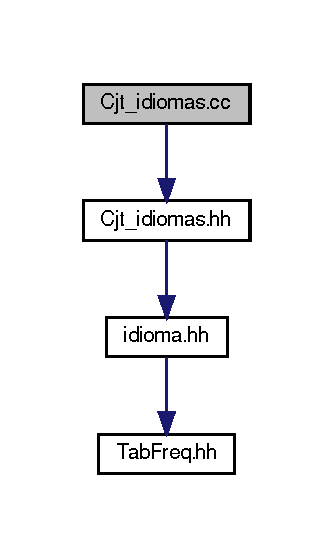
\includegraphics[width=160pt]{_cjt__idiomas_8cc__incl}
\end{center}
\end{figure}


\subsection{Descripción detallada}
Implementación de la clase \hyperlink{_cjt__idiomas_8hh}{Cjt\+\_\+idiomas.\+hh}. 


\hypertarget{_cjt__idiomas_8hh}{}\section{Referencia del Archivo Cjt\+\_\+idiomas.\+hh}
\label{_cjt__idiomas_8hh}\index{Cjt\+\_\+idiomas.\+hh@{Cjt\+\_\+idiomas.\+hh}}


Especificación de la clase \hyperlink{class_cjt__idiomas}{Cjt\+\_\+idiomas}.  


Dependencia gráfica adjunta para Cjt\+\_\+idiomas.\+hh\+:
\nopagebreak
\begin{figure}[H]
\begin{center}
\leavevmode
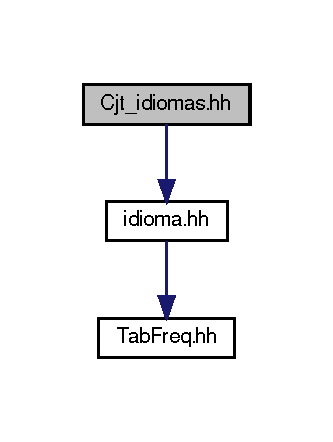
\includegraphics[width=160pt]{_cjt__idiomas_8hh__incl}
\end{center}
\end{figure}
\subsection*{Clases}
\begin{DoxyCompactItemize}
\item 
class \hyperlink{class_cjt__idiomas}{Cjt\+\_\+idiomas}
\begin{DoxyCompactList}\small\item\em Representa un conjunto de idiomas. \end{DoxyCompactList}\end{DoxyCompactItemize}


\subsection{Descripción detallada}
Especificación de la clase \hyperlink{class_cjt__idiomas}{Cjt\+\_\+idiomas}. 


\hypertarget{idioma_8cc}{}\section{Referencia del Archivo idioma.\+cc}
\label{idioma_8cc}\index{idioma.\+cc@{idioma.\+cc}}


Implementación de la clase \hyperlink{idioma_8hh}{idioma.\+hh}.  


Dependencia gráfica adjunta para idioma.\+cc\+:
\nopagebreak
\begin{figure}[H]
\begin{center}
\leavevmode
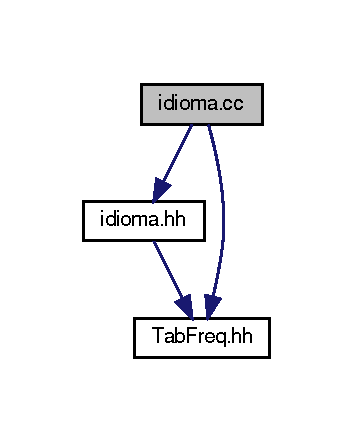
\includegraphics[width=170pt]{idioma_8cc__incl}
\end{center}
\end{figure}
\subsection*{Funciones}
\begin{DoxyCompactItemize}
\item 
bool \hyperlink{idioma_8cc_ae4068cab7e1ad43a8d03f2f5d50e06df}{operator$<$} (const Bin\+Tree$<$ pair$<$ string, int $>$$>$ \&a, const Bin\+Tree$<$ pair$<$ string, int $>$$>$ \&b)
\end{DoxyCompactItemize}


\subsection{Descripción detallada}
Implementación de la clase \hyperlink{idioma_8hh}{idioma.\+hh}. 



\subsection{Documentación de las funciones}
\mbox{\Hypertarget{idioma_8cc_ae4068cab7e1ad43a8d03f2f5d50e06df}\label{idioma_8cc_ae4068cab7e1ad43a8d03f2f5d50e06df}} 
\index{idioma.\+cc@{idioma.\+cc}!operator$<$@{operator$<$}}
\index{operator$<$@{operator$<$}!idioma.\+cc@{idioma.\+cc}}
\subsubsection{\texorpdfstring{operator$<$()}{operator<()}}
{\footnotesize\ttfamily bool operator$<$ (\begin{DoxyParamCaption}\item[{const Bin\+Tree$<$ pair$<$ string, int $>$$>$ \&}]{a,  }\item[{const Bin\+Tree$<$ pair$<$ string, int $>$$>$ \&}]{b }\end{DoxyParamCaption})}



Definición en la línea 208 del archivo idioma.\+cc.


\begin{DoxyCode}
208                                                                                        \{
209   pair<string,int> p\_a = a.value();
210   pair<string,int> p\_b = b.value();
211 
212   \textcolor{keywordflow}{if} (p\_a.second == p\_b.second)\{
213     \textcolor{keywordflow}{return} (p\_a.first < p\_b.first);
214   \}\textcolor{keywordflow}{else} \textcolor{keywordflow}{return} (p\_a.second < p\_b.second);
215 \}
\end{DoxyCode}

\hypertarget{idioma_8hh}{}\section{Referencia del Archivo idioma.\+hh}
\label{idioma_8hh}\index{idioma.\+hh@{idioma.\+hh}}


Especificación de la clase \hyperlink{class_idioma}{Idioma}.  


Dependencia gráfica adjunta para idioma.\+hh\+:
\nopagebreak
\begin{figure}[H]
\begin{center}
\leavevmode
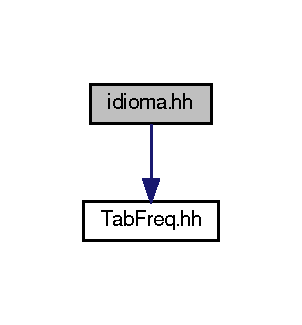
\includegraphics[width=145pt]{idioma_8hh__incl}
\end{center}
\end{figure}
\subsection*{Clases}
\begin{DoxyCompactItemize}
\item 
class \hyperlink{class_idioma}{Idioma}
\begin{DoxyCompactList}\small\item\em Representa un idioma. \end{DoxyCompactList}\end{DoxyCompactItemize}


\subsection{Descripción detallada}
Especificación de la clase \hyperlink{class_idioma}{Idioma}. 


\hypertarget{program_8cc}{}\section{Referencia del Archivo program.\+cc}
\label{program_8cc}\index{program.\+cc@{program.\+cc}}


Programa principal de la práctica.  


Dependencia gráfica adjunta para program.\+cc\+:
\nopagebreak
\begin{figure}[H]
\begin{center}
\leavevmode
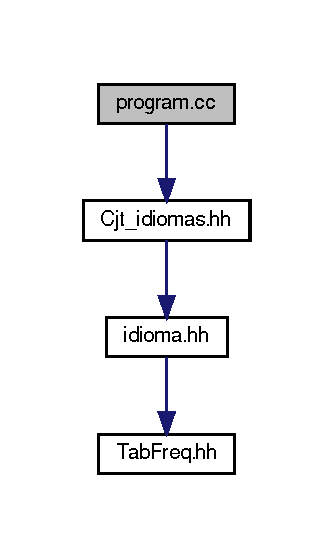
\includegraphics[width=160pt]{program_8cc__incl}
\end{center}
\end{figure}
\subsection*{Funciones}
\begin{DoxyCompactItemize}
\item 
int \hyperlink{program_8cc_ae66f6b31b5ad750f1fe042a706a4e3d4}{main} ()
\end{DoxyCompactItemize}


\subsection{Descripción detallada}
Programa principal de la práctica. 



\subsection{Documentación de las funciones}
\mbox{\Hypertarget{program_8cc_ae66f6b31b5ad750f1fe042a706a4e3d4}\label{program_8cc_ae66f6b31b5ad750f1fe042a706a4e3d4}} 
\index{program.\+cc@{program.\+cc}!main@{main}}
\index{main@{main}!program.\+cc@{program.\+cc}}
\subsubsection{\texorpdfstring{main()}{main()}}
{\footnotesize\ttfamily int main (\begin{DoxyParamCaption}{ }\end{DoxyParamCaption})}



Definición en la línea 19 del archivo program.\+cc.


\begin{DoxyCode}
19            \{
20   \textcolor{keywordtype}{int} NI; \textcolor{comment}{//NI es nombre de idiomes}
21   \textcolor{keywordtype}{string} opcio;
22   cin >> NI;
23   \hyperlink{class_cjt__idiomas}{Cjt\_idiomas} c1;
24   c1.\hyperlink{class_cjt__idiomas_a09e45083b9df57c02f05bda0bef3d0d3}{read\_conjunto}(NI);
25   cin >> opcio;
26   \textcolor{keywordflow}{while}(opcio != \textcolor{stringliteral}{"fin"})\{
27     \textcolor{keywordflow}{if} (opcio == \textcolor{stringliteral}{"anadir/modificar"})\{
28       \textcolor{keywordtype}{string} nomI;
29       cin >> nomI;
30       c1.\hyperlink{class_cjt__idiomas_a1e38b16ba4bb49a91589c85ec7775a5f}{afegir\_mod\_idioma}(nomI);
31     \}
32 
33     \textcolor{keywordflow}{else} \textcolor{keywordflow}{if} (opcio == \textcolor{stringliteral}{"codifica"})\{
34       \textcolor{keywordtype}{string} text, nomI;
35       cin >> nomI >> text;
36       c1.\hyperlink{class_cjt__idiomas_af3724a3343435acc48397c555722ce2f}{codifica\_I}(nomI,text);
37     \}
38 
39     \textcolor{keywordflow}{else} \textcolor{keywordflow}{if} (opcio == \textcolor{stringliteral}{"decodifica"})\{
40       \textcolor{keywordtype}{string} codi, nomI;
41       cin >> nomI >> codi;
42       c1.\hyperlink{class_cjt__idiomas_a99a44238cc4b83392ff1991ad1319c46}{decodifica\_I}(nomI,codi);
43     \}
44 
45     \textcolor{keywordflow}{else} \textcolor{keywordflow}{if} (opcio == \textcolor{stringliteral}{"tabla\_frec"})\{
46       \textcolor{keywordtype}{string} nomI;
47       cin >> nomI;
48       c1.\hyperlink{class_cjt__idiomas_a9839ea44dc8c3ecbb10b32fe869a3498}{print\_taula}(nomI);
49       \}
50 
51     \textcolor{keywordflow}{else} \textcolor{keywordflow}{if} (opcio == \textcolor{stringliteral}{"treecode"})\{
52       \textcolor{keywordtype}{string} nomI;
53       cin >> nomI;
54       c1.\hyperlink{class_cjt__idiomas_abcb2442285737fae69096a5e05b9a594}{print\_I\_treecode}(nomI);
55     \}
56 
57     \textcolor{keywordflow}{else} \textcolor{keywordflow}{if} (opcio == \textcolor{stringliteral}{"codigos"})\{
58       \textcolor{keywordtype}{string} nomI, opcio2;
59       cin >> nomI >> opcio2;
60       \textcolor{keywordflow}{if} (opcio2 == \textcolor{stringliteral}{"todos"})
61         c1.\hyperlink{class_cjt__idiomas_a0ac0bb2a2fe0cf4abd10d9366da9fa10}{print\_lista}(nomI);
62       \textcolor{keywordflow}{else} c1.\hyperlink{class_cjt__idiomas_afb0c806ea9fb7422f10d7767ef101743}{print\_code\_op}(nomI,opcio2);
63     \}
64     cin >> opcio;
65   \}
66 \}
\end{DoxyCode}

\hypertarget{_tab_freq_8cc}{}\section{Referencia del Archivo Tab\+Freq.\+cc}
\label{_tab_freq_8cc}\index{Tab\+Freq.\+cc@{Tab\+Freq.\+cc}}


Implementación de la clase \hyperlink{_tab_freq_8hh}{Tabfreq.\+hh}.  


Dependencia gráfica adjunta para Tab\+Freq.\+cc\+:
\nopagebreak
\begin{figure}[H]
\begin{center}
\leavevmode
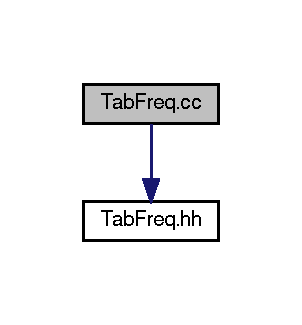
\includegraphics[width=145pt]{_tab_freq_8cc__incl}
\end{center}
\end{figure}


\subsection{Descripción detallada}
Implementación de la clase \hyperlink{_tab_freq_8hh}{Tabfreq.\+hh}. 


\hypertarget{_tab_freq_8hh}{}\section{Referencia del Archivo Tab\+Freq.\+hh}
\label{_tab_freq_8hh}\index{Tab\+Freq.\+hh@{Tab\+Freq.\+hh}}


Especificación de la clase \hyperlink{class_tab_freq}{Tab\+Freq}.  


\subsection*{Clases}
\begin{DoxyCompactItemize}
\item 
class \hyperlink{class_tab_freq}{Tab\+Freq}
\begin{DoxyCompactList}\small\item\em Representa una tabla de frecuencias de los carácteres de un idioma. \end{DoxyCompactList}\end{DoxyCompactItemize}


\subsection{Descripción detallada}
Especificación de la clase \hyperlink{class_tab_freq}{Tab\+Freq}. 


%--- End generated contents ---

% Index
\backmatter
\newpage
\phantomsection
\clearemptydoublepage
\addcontentsline{toc}{chapter}{Índice}
\printindex

\end{document}
